\documentclass[twoside]{report}
\usepackage{algorithm}
\usepackage{algorithmicx}
\usepackage{algpseudocode}
%% Data:  2015-04-19
%% Author: Abolfazl Diyanat

%%% ================================================================================================== اضافه کردن یکسری بسته‌های پایه
%% در مورد تقدم و تاخر وارد کردن بسته ها تنها باید به چند نکته دقت کرد:
%% الف) بسته xepersian حتما حتما باید آخرین بسته ای باشد که فراخوانی می شود، به استثنای بسته  های bidi
%% ب) بسته hyperref جزو آخرین بسته هایی باید باشد که فراخوانی می شود.
%% ج) بسته glossaries حتما باید بعد از hyperref فراخوانی شود. 
%% د) بسته listings باید حتما قبل از  hyperref فراخوانی شود. 

\usepackage{etex}
\reserveinserts{28}

%%% تمام بسته های مورد نیاز برای  کارهای ریاضیاتی به صورت کامل اینجا آورده شده است در صورتی که بخواهید از بسته های دیگر استفاده کنید بهتر است که آن‌ها را به گونه ای انتخاب کنید که با این بسته ها تداخل نداشته باشد. به نظر من استفاده از همین بسته ها کافی است.
%%% amsthm: It introduces the proof environment and the \theoremstyle command.
%%%  amssymb: It adds new symbols in to be used in math mode.
%%% amsmath: It contains the advanced math extensions for LaTeX. The complete documentation should be in your LaTeX distribution; the file is called amsdoc, and can be dvi or pdf.

\usepackage{amsthm,amssymb,amsmath}
\usepackage{thmtools}
\usepackage{dsfont}
\usepackage{fancyhdr}

%%% بسته‌ای برای فعال‌سازی پارامتر H در وارد کردن شکل. این پارامتر شکل را در همان‌جایی که دقیقا فراخوانی کرده‌ایم، وارد می‌کند.
\usepackage{float}

%%% برای تنظیم حاشیه صفحات
\usepackage{geometry}

% بسته ای برای تنظیم فونت، اندازه و نحوه نمایش caption
\usepackage{caption}
\usepackage{subcaption}

%%% بسته‌ای برای تنظیم حاشیه و کادر دور فرمول و ... 
\usepackage{empheq,fancybox}

%%% برای رنگی کردن متن و استفاده از رنگ در متن این دو بسته مورد نیاز است.
\usepackage[usenames,dvipsnames]{color,xcolor}

%%% It extends the possibility of LaTeX to handle tables, fixing some bugs and adding new features. Using it, you can create very complicated and customized tables. For more information, see the Tables section.
\usepackage{array}

%%% بسته ای برای استفاده از اشکال برای آیتم‌ها
\usepackage{pifont}

\usepackage{booktabs}
\setlength{\heavyrulewidth}{1.5pt}
\setlength{\abovetopsep}{4pt}

%%% بسته‌ای برای رسم اشکال و تصاویر با Latex
\usepackage{tikz}
\usetikzlibrary{calc}

\RequirePackage[framemethod=TikZ]{mdframed}

\usepackage[explicit]{titlesec}

%% Line spacing
%%To change line spacing in the whole document use the command \linespread covered in Text Formatting.
% %To change line spacing in specific environments use setspace
\usepackage{setspace}

%%% بسته ای برای وارد کردن الگوریتم در متن
%\usepackage{algorithm}
%\usepackage{algorithmicx}
%\usepackage{algpseudocode}


%%% در این قالب از بسته graphx برای انجام کارهای گرافیکی استفاده می‌شود. این بسته برای اضافه کردن تصویرها به متن استفاده شده است.
\usepackage{graphicx}

%%% دوبسته برای اضافه کردن دستورات if و else به برنامه.
\usepackage{xparse,ifthen}

\usepackage{colortbl}

%%% بسته ای برای وارد کردن کدهای برنامه نویسی (MATLAB، JAVA و ...) در متن. بسته listings باید قبل از hyperref باشد و گرنه با خطا مواجه خواهیم شد. برای مطالب بیشتر در مورد نحوه کارکرد این بسته سایت زیر را مشاهده کنید.
%%% http://www.parsilatex.com/mediawiki/index.php?title=%D8%B1%D8%A7%D9%87%D9%86%D9%85%D8%A7%DB%8C_%D9%88%D8%A7%D8%B1%D8%AF_%DA%A9%D8%B1%D8%AF%D9%86_%DA%A9%D8%AF_%D8%AF%D8%B1_%D9%85%D8%AA%D9%86
\usepackage{listings}

\usepackage{makeidx}
\makeindex

\usepackage{etoolbox}

%%% بسته ای برای رنگی کردن لینک ها و فعال سازی لینک ها در یک نوشتار، بسته hyperref باید جزو آخرین بسته‌هایی باشد که فراخوانی می‌شود. 
\usepackage{hyperref}


%%% بسته‌ای برای وارد کردن واژه نامه در متن، این بسته باید بعد از hyperref حتما صدا زده شود. 
\usepackage[xindy,acronym,nonumberlist=true]{glossaries}
%%%زی‌پرشین (به انگلیسی: XePersian) یک بسته حروف‌چینی رایگان و متن‌باز برای نگارش مستندات پارسی/انگلیسی با زی‌لاتک است.
%%% در واقع، زی‌پرشین، کمک می‌کند تا به آسانی، مستندات را به پارسی، حروف‌چینی کرد. این بسته را وفا خلیقی نوشته است،
%%% و به طور منظم، آن را بروز‌رسانی کرده و باگ‌های آن را رفع می‌کند.
%%% نکته مهم این جا است که بسته Xepersian برای پشتیبانی از زبان فارسی آورده شده است، و 
%%% می بایست آخرین بسته ای باشد که شما وارد می کنید، دقت کنید: آخرین بسته 
\usepackage[extrafootnotefeatures]{xepersian}

%% توسط دستور \myData می توانید تاریخ و ساعت را وارد متن خود کنید. 
\newcommand{\myData}{
	\newcount \hour
	\newcount \min
	\newcommand*{\timeoftoday}{%
		\hour\time\divide\hour 60 ساعت \the\hour{}
		\min\time\multiply\hour 60 \advance\min-\hour
		\ifnum\min=0
		\else
		و
		\the\min{} دقیقه
		\fi}
	\today{} در \timeoftoday
} %M



%%% =========================================================================================================================

%%% اضافه کردن نماد استقلال به علایم ریاضی
\newcommand{\Perp}{\perp \! \! \! \perp}
\newcommand{\independent}{\protect\mathpalette{\protect\independenT}{\perp}} \def\independenT#1#2{\mathrel{\rlap{$#1#2$}\mkern2mu{#1#2}}}

%%% این دستور به این خاطر تعریف می‌شود، که اگر بخواهیم مثلا یک کلمه در واژه نامه را Index‌کنیم، مثلا بنویسیم، ‎\index{\glspl{Water}‎}‎، این دستور index درست عمل نمی‌کند. نویسنده بسته glossaries در این باره این طور گفته است.
%%%If you inspect the .idx file you will see that it contains the following:
%%%\indexentry{\glsentryplural{StrictlyStable}|hyperpage}{1}
%%%\index doesn't expand its argument when writing to the .idx file and since xindy doesn't understand (La)TeX commands the index won't be correctly sorted. This is a feature of \index and is not connected with glossaries.
%%%You could try something like
%%%\expandafter\index\expandafter{\glsentryplural{StrictlyStable}}
%%% توسط دستور تعیین شده می‌توان این مشکل را حل کرد. دقت کنید که این دستور می‌بایست حتما برای واژه‌نامه ها فقط تعریف شود.

%\let\oldindex\index
%\renewcommand{\index}[1]{
%\ifthenelse{\equal{\glsentrytype{#1}}{english}}
	%{\expandafter\oldindex\expandafter{\glsentrytext{#1}}}
	%{ \ifthenelse{\equal{\glsentrytype{#1}}{acronym}}
		%{\expandafter\oldindex\expandafter{\glsentrytext{#1}}}
		%{\oldindex{#1}}
	%}
%}

%%% گاهی اوقات مطلبی را در یک بخش، فصل و ... می‌نویسیم، وقتی این مطلب را در متن ارجاع می دهیم، مثلا می نویسیم بخش ‎\ref{seclabel}‎، اما ممکن است به هر علتی مطلب ما از بخش به فصل و یا به یک زیربخش تنزل پیدا کند.
%%% بدین‌منظور به جای دستور ref از autoref استفاده می‌کنیم. در این صورت خود latex می‌فهمد که این مطالب در ‎چه قسمتی است و خودش کلمه فصل، بخش و یا ... را قبل از شماره آن اضافه می‌کند. دستورات زیر می‌گوید در هر یک 
%%% از سطوح متن چه کلمه‌ای‌ قرار گیرد. 
\def\sectionautorefname{بخش}
\def\subsectionautorefname{زیربخش}
\def\subsubsectionautorefname{زیربخش}


% حل شدن مشکل part
%%%% تعریف یکسری دستور به منظور حل مشکل قرار دادن part در متن و آمدن آن در فهرست مطالب. 
\makeatletter
\renewcommand*\l@part[2]{
	\ifnum \c@tocdepth >-2\relax
	\addpenalty{-\@highpenalty}
	\addvspace{2.25em \@plus\p@}
	\setlength\@tempdima{3em}
	\begingroup
	\parindent \z@ \if@RTL\leftskip\else\rightskip\fi \@pnumwidth
	\parfillskip -\@pnumwidth
	{\leavevmode
		\large \bfseries\textcolor{blue}{بخش} #1
		\hfil \hb@xt@\@pnumwidth{\hss #2}}\par
	\nobreak
	\global\@nobreaktrue
	\everypar{\global\@nobreakfalse\everypar{}}
	\endgroup
	\fi}
\makeatother

\makeatletter
\def\@chapter[#1]#2{\ifnum \c@secnumdepth >\m@ne
	\if@mainmatter
	\refstepcounter{chapter}%
	\typeout{\@chapapp\space\thechapter.}%
	\addcontentsline{toc}{chapter}%
	{\@chapapp~\protect\numberline{\arabic{chapter}}~~~ #1}%
	\else
	\addcontentsline{toc}{chapter}{#1}%
	\fi
	\else
	\addcontentsline{toc}{chapter}{#1}%
	\fi
	\chaptermark{#1}%
	%\addtocontents{lof}{\protect\addvspace{10\p@}}%
	%\addtocontents{lot}{\protect\addvspace{10\p@}}%
	\if@twocolumn
	\@topnewpage[\@makechapterhead{#2}]%
	\else
	\@makechapterhead{#2}%
	\@afterheading
	\fi}
%\renewcommand*\l@section{\@dottedtocline{1}{4.5em}{2.3em}}
%\renewcommand*\l@subsection{\@dottedtocline{2}{6.5em}{3.2em}} 
\makeatother

%%% این دستور به این خاطر تعریف می‌شود، که اگر بخواهیم مثلا یک کلمه در واژه نامه را Index‌کنیم، مثلا بنویسیم، ‎\index{\glspl{Water}‎}‎، این دستور index درست عمل نمی‌کند. نویسنده بسته glossaries در این باره این طور گفته است.
%%%If you inspect the .idx file you will see that it contains the following:
%%%\indexentry{\glsentryplural{StrictlyStable}|hyperpage}{1}
%%%\index doesn't expand its argument when writing to the .idx file and since xindy doesn't understand (La)TeX commands the index won't be correctly sorted. This is a feature of \index and is not connected with glossaries.
%%%You could try something like
%%%\expandafter\index\expandafter{\glsentryplural{StrictlyStable}}
%%% توسط دستور تعیین شده می‌توان این مشکل را حل کرد. دقت کنید که این دستور می‌بایست حتما برای واژه‌نامه ها فقط تعریف شود. 
\newcommand{\indexglspl}[1]{\expandafter\index\expandafter{\glsentryplural{#1}}}
\newcommand{\indexgls}[1]{\expandafter\index\expandafter{\glsentryname{#1}}}


%%% 0000000000000000000000000000000000000000000000000000000000000000000000000000000000000000000000000000000000000000000000000000000000000000 
%%%==================== تنظیمات بسته geometry
%%% تنظیمات مربوط به حاشیه صفحه
\geometry{a4paper,top=30mm, bottom=20mm, right=30mm,left=20mm}
% %%% در Latex انواع مختلفی از اندازه‌ها برای ابعاد کاغذ وجود دارد. گرچه شما می‌توانید به دلخواه ابعاد مختلفی به کاغذ بدهید. 
%%%%a0paper, a1paper, a2paper, a3paper, a4paper, a5paper, a6paper,b0paper, b1paper, b2paper, b3paper, b4paper, b5paper, b6paper, c0paper, c1paper, c2paper, c3paper, c4paper, c5paper, c6paper, b0j, b1j, b2j, b3j, b4j, b5j, b6j, ansiapaper, ansibpaper, ansicpaper, ansidpaper, ansiepaper, letterpaper, executivepaper, legalpaper

%%% 0000000000000000000000000000000000000000000000000000000000000000000000000000000000000000000000000000000000000000000000000000000000000000 
%%==================== تنظیمات hyperref

%%% برای وارد کردن کلمه (بخش) در فهرست مطالب بسته hyperref برای حالت فارسی یک مشکل دارد. بدین منظور این 
%%% مشکل را به صورت دستی حل شده است. برای این که رنگ keywordstyle که تعیین کننده رنگ کل قسمت فهرست مطالب
%%% نیز هست یکسان در آید یک پارامتر رنگ برای keywordstyle این جا تعریف می‌کنیم، و سپس از آن هم در تنظمیات hypperref 
%%% و هم در اون کدهایی که به صورت دستی وارد شده است، استفاده می‌شود.  مطالب بیشتر در مورد این بسته را در سایت زیر مطالعه کنید.
%%% http://en.wikibooks.org/wiki/LaTeX/Hyperlinks

%% در این قسمت تنظیمات بسته hyperref را قرار می دهیم.
%% این تنظیمات شامل موارد زیر است:

\hypersetup{
	pdfmenubar=false,			% show or hide Acrobat’s menu
	pdftoolbar=true,			%show or hide Acrobat’s toolbar
%% موقعی که فایل پی دی اف خروجی را باز می کنید صفحه به صورت عریض و بزرگ باز می شود.
	pdfstartview=FitH, 
	%% مواردی که برای فعال سازی این که شماره اشکال را به صورت ارجاعی نشان دهد
	%hyperfigures=true,
	%% به جای استفاده از مربع قرمز دور موارد ارجاعی از لینک های رنگی استفاده کند.
	colorlinks=true, 
	%% رنگ برخی از لینک ها در زیر تعریف شده است. 
	linkcolor=blue, 
	anchorcolor=green, 
	citecolor=magenta, 
	urlcolor=cyan, 
	filecolor=magenta, 
	bookmarkstype=toc,
	unicode = true			%allows to use characters of non-Latin based languages in Acrobat’s bookmarks
	%bookmarksopen = true,
	%bookmarksopenlevel = 1
	%%% اگر این option را true‌ بکنیم، آن‌گاه در کنار bookmark شماره فصل و بخش و زیربخش نیز می آید. مثلا می‌نویسد: ۱.۲ طراحی شبکه
	%bookmarksnumbered = true,
	%hidelinks			%hide links (removing color and border)
} % M



%% 0000000000000000000000000000000000000000000000000000000000000000000000000000000000000000000000000000000000000000000000000000000000000000 

%%==================== تنظیمات algorithm و algorithmic
%\floatname{algorithm}{الگوریتم}

%% 0000000000000000000000000000000000000000000000000000000000000000000000000000000000000000000000000000000000000000000000000000000000000000 
%% تنظیم فونت. 
%%برای دانستن اطلاعات بیشتر در مورد تنظیم فونت به لینک زیر مراجعه کنید.
%%http://www.parsilatex.com/mediawiki/index.php?title=%D9%81%D9%88%D9%86%D8%AA_%D8%AF%D8%B1_xepersian
%% دقت شود که در این استایل از فونت های زیر استفاده می‌شود، بدین‌سان لازم است فونت هایی که فعال هستند (comment نیستند) توسط کاربر در سیستم عامل نصب شود.
%%سعی شده است از فونت های استاندارد IR‌ که حاصل کار شورای عالی اطلاع رسانی هست، استفاده شود، کاربران می‌توانند فونت های یاد شده را از لینک زیر دانلود کنند.
%% http://www.scict.ir/portal/Home/Default.aspx?CategoryID=b50ee619-ce53-4c25-bf53-b0f0332c1777

%% تعریف یک دستور به عنوان فونت پیش فرض
\newcommand{\defaultFont}{
	%%  با دستور زیر می توانید فونتی مخصوص عبارات فارسی تعیین کنید:
	\settextfont[Scale=1.3]{IRNazanin}
	%% شما با دستور زیر بعد از فراخوانی بسته xepersian می توانید فونت انگلیسی را تعیین کنید
	%% دقت کنید که عبارات انگلیسی شما باید در دستور \lr{} قرار گیرد تا xepersian بتواند بفمهد که این عبارات انگلیسی است
	\setlatintextfont[Scale=1]{Times New Roman}
	%% تعریف برای فونت اعداد و ارقام
	%\setdigitfont[Scale=1.1]{XB Zar}
} % M

\defaultFont

%% توسط دستورات defpersianfont و deflatinfont به ترتیب می توان یکسری فونت فارسی و انگلیسی دیگر تعریف کرد که در جاهای دیگر متن بتوان از آن استفاده کرد. برای استفاده کافی است که عبارتی که می خواهیم فونت آن عوض شود را به صورت زیر به عنوان نمونه بنویسیم.
%% \versionfont{این یک مثال است. }
%%% فونت عنوان گزارش
\defpersianfont\titlefont[Scale=2.4]{IRTitr}
\defpersianfont\logofontR[Scale=1.2]{Zar}
\defpersianfont\typefontR[Scale=1.8]{Zar}
\defpersianfont\titlefontR[Scale=2]{Titr}
\defpersianfont\datafontR[Scale=1.4]{B Zar}
\defpersianfont\proposalFont[Scale=1]{Titr}
\defpersianfont\InstituteFont[Scale=.8]{XM Traffic}
\defpersianfont\godFont[Scale=.9]{XM Traffic}
\defpersianfont\nastaliq[Scale=2]{IranNastaliq}

%%  با استفاده از این دستور می‌توان فونت و فارسی و یا انگلیسی بودن اعداد در فرمول‌ها را به حالت اولیه (یعنی پیش‌فرض لاتک) برگرداند.
\DefaultMathsDigits

%% نحوه تغییر اندازه فونت عبارات ریاضی و فرمول‌ها. این کار توسط دستور زیر انجام می‌شود. 
%%\DeclareMathSizes{textsize}{mathsize}{scriptsize}{scriptscriptsize}
%% گزینه اول: این برای چه دسته فونتی است. پیش فرض استایل ما فونت 10pt است. 
%% گزینه دوم: اندازه فونت توابع و موجودات ریاضی درون متن.
%% گزینه سوم: برای اسکریپت ها، اندازه زیرنویس و بالانویس.
%% گزینه چهارم: برای زیرنویس زیرنویس.


%%% =========================================================================================================



%% فایل  Environments  در برگیرنده تعریف یکسری استایل برای فصل‌ها است. 
%%% Last Update: 24 Jul 2019
%

%% =========================================================================================================================
% انواع مختلف استایل‌های برای عنوان فصل‌ها 

\newcommand*\chapterlabel{}
\titleformat{\chapter}
  {\gdef\chapterlabel{}
   \normalfont\Huge\bfseries}
  {\gdef\chapterlabel{\thechapter\ }}{0pt}
  {\begin{tikzpicture}[remember picture,overlay]
    \node[yshift=-3cm] at (current page.north west)
      {\begin{tikzpicture}[remember picture, overlay]
        \draw[fill=BlueGreen] (0,0) rectangle
          (\paperwidth,3cm);
        \setRTL
        \node[anchor=east,xshift=0.95\paperwidth,rectangle,
              rounded corners=20pt,inner sep=11pt,
              fill=MidnightBlue,text width=\dimexpr0.9\paperwidth-22pt\relax,align=justify]
             {\addfontfeature{Color=F5F5F5}\chapterlabel#1};
       \end{tikzpicture}
      };
   \end{tikzpicture}
  }
%\titlespacing*{\chapter}{0pt}{50pt}{-60pt}
\makeatletter
\bidi@patchcmd{\@makechapterhead}%
{\huge\bfseries\@chapapp\space\thechapter}%
{}%
{}
{}

\bidi@patchcmd{\@chapter}%
{\addcontentsline{toc}{chapter}{\protect\numberline{\thechapter}#1}}%
{\addcontentsline{toc}{chapter}{#1}}%
{}
{}

\bidi@patchcmd{\@part}{%
  \addcontentsline{toc}{part}{\thepart\hspace{1em}#1}%%
}{%
  \addtocontents{toc}{\bfseries\protect\centering\thepart\hspace{1em}#1\par}%
}{}{}
\makeatother




%%% تعریف یکسری استایل برای صفحه شروع 
%% Last Update: 20 Sep 2019
%

%% =================================================================================
\makeatletter
% تعریف یکسری متغیرها که کاربر می‌تواند بعدا آن ها را مقداردهی کند. 

\gdef\@type{نوع پروژه}
\def\type#1{\gdef\@type{#1}}

% عنوان محصول را تعیین می‌کند. این عنواند در ایجاد عنوان در مستند استفاده می‌شود این عنوان در هر مستند باید ایجاد شود در غیر این صورت از عنوان پیشفرض استفاده خواهد شد.
\gdef\@title{عنوان پروژه}
\def\title#1{\gdef\@title{#1}}

% زیر عنوان یک متن ساده را تعیین می‌کند که یک هدف مهم محصول را تعیین می‌کند این عنوان می تواند برای یک محصول در نظر گرفته نشود. از این داده برای  ایجاد عنوان و سایر مکان های محصول استفاده می‌شود.
\gdef\@subtitle{کاربرد محصول برای استفاده در زیر عنوان}
\def\subtitle#1{\gdef\@subtitle{#1}}
% افراد و گروه های که در تهیه این مستند و محصول همکاری داشته اند را تعیین می کند این داده همواره باید بیان شود. این داده در نوشتن عنوان و دیگر قسمت های مستند مورد استفاده قرار می‌گیرد.
\gdef\@author{}
\def\author#1{\gdef\@author{#1}}
\newcommand{\authorText}{\@author\,}
% تاریخ نهایی نوشتن مستند را تعیین می‌کند این تاریخ در نوشتن عنوان استفاده می‌شود این تارخ باید تعیین شود در غیر این صورت به صورت پیش فرض یک تاریخ برای آن استفاده می شود.
\gdef\@date{ آخرین ویرایش: \myData}
\def\date#1{\gdef\@date{#1}}

\gdef\@supervisor{} 
\def\supervisor#1{\gdef\@supervisor{#1}}
\newcommand{\supervisorText}{\@supervisor\,}

\gdef\@adviser{نام استاد مشاور}
\def\adviser#1{\gdef\@adviser{#1}}

\gdef\@session{جلسه ارایه}
\def\session#1{\gdef\@session{#1}}

\gdef\@institute{پژوهشکده}
\def\institute#1{\gdef\@institute{#1}}

\gdef\@faculity{ نام دانشکده}
\def\faculity#1{\gdef\@faculity{#1}}

\gdef\@group{ نام گروه}
\def\group#1{\gdef\@group{#1}}

\gdef\@community{نام زیرگروه}
\def\community#1{\gdef\@community{#1}}

\gdef\@forwhat{پایان‌نامه یا رساله برای دریافت درجه}
\def\forwhat#1{\gdef\@forwhat{#1}}

\gdef\@field{در رشته مهندسی کامپیوتر گرایش}
\def\field#1{\gdef\@field{#1}}

\gdef\@version{اول}
\def\version#1{\gdef\@version{#1}}

% نام فایلی لوگوی مورد استفاده در نوشتار توسط این پارامتر مشخص می‌شود. 
\gdef\@logofile{logonotfound}
\def\logofile#1{\gdef\@logofile{#1}}
% اندازه فایل لوگوی موجود در متن توسط این پارامتر مشخص می‌شود.
\gdef\@logoScale{.3\textwidth}
\def\logoScale#1{\gdef\@logoScale{#1}}


%% ============================================================================================================================
%  برگه نخست در مستند را ایجاد می‌کند. در این برگه تنها نام پروردگار  ذکر می‌شود. برای ایجاد نام پرودگار یک تصویر استفاده می‌شود به نام god.ps  که باید در پوشه image کنار پرونده اصلی مستند قرار گرفته شده باشد.
\deflatinfont\besm[Scale=50]{Besmellah 2}
\DeclareDocumentCommand{\Godpage}{g g}{	
	\thispagestyle{empty}
	\begin{center}
	\IfValueTF{#1}{
		\IfValueTF{#2}{
			\includegraphics[width=#2\textwidth]{#1}
		}{%
			\includegraphics[width=.7\textwidth]{#1}
		}%
	}{%%
		\IfValueTF{#2}{
			{\besm #2}
		}{%
			{\besm b}

		}%
	}%%
	\end{center}
	\newpage
}%

\DeclareDocumentCommand{\Godpage}{g}{	
	\thispagestyle{empty}
	\begin{center}
		\IfValueTF{#1}{
			{\besm #1}
		}{%
			{\besm f}

		}%
	\end{center}
	\newpage
}%

\DeclareDocumentCommand{\GodpageFont}{gg}{	
	\thispagestyle{empty}
	\begin{center}
		\IfValueTF{#1}{
			\IfValueTF{#2}{
			}{%
			}%
			{\besm بسم‌الله الرحمن الرحیم}
		}{%
			{\besm بسم‌الله الرحمن الرحیم}

		}%
	\end{center}
	\newpage
}%


%% ============================================================================================================================

\newcommand{\pejoheshStyle}{
% این یک استایل ساده و رسمی.
% توسط این دستور تمامی footer و header های صفحه را حذف می‌کنیم. 
	\thispagestyle{empty}
	\begin{center}
		\includegraphics[width=\@logoScale]{\@logofile}\\*[10pt]
		\logofontR{\@institute}\medskip
		\vspace*{\stretch{2}}
		\typefontR\textbf{\@type}\\*[35pt]
		\titlefontR\textbf{\@title}\medskip
		\vspace*{\stretch{2}}
		\datafontR{\@author}\medskip
		\vspace*{\stretch{2}}
		\datafontR{\@date}
		\vspace*{\stretch{1}}
	\end{center}
	\clearpage
} %


%% ============================================================================================================================
% توسط دستورات defpersianfont و deflatinfont به ترتیب می توان یکسری فونت فارسی و انگلیسی دیگر تعریف کرد که در جاهای دیگر متن بتوان از آن استفاده کرد. برای استفاده کافی است که عبارتی که می خواهیم فونت آن عوض شود را به صورت زیر به عنوان نمونه بنویسیم.
\defpersianfont\titlefont[Scale=2.4]{IRTitr}
\newcommand{\lshortStyle}{
% استایلی شبیه به استایل شروع کتاب "مقدمه‌ای نه چندان کوتاه بر Latex"
	\definecolor{authorcol}{rgb}{.51,0,.51}
	\begin{flushleft}
	\vspace*{\stretch{.1}}
	\begin{flushright}\includegraphics[width=\@logoScale]{\@logofile}\end{flushright}
	\newlength{\centeroffset}
	\setlength{\centeroffset}{-0.5\oddsidemargin}
	\addtolength{\centeroffset}{0.5\evensidemargin}
	\addtolength{\textwidth}{-\centeroffset}
% توسط این دستور تمامی footer و header های صفحه را حذف می‌کنیم. 
	\thispagestyle{empty}
	
	\vspace*{\stretch{2}}
	
	\noindent\hspace*{\centeroffset}\makebox[0pt][l]{
		\begin{minipage}{\textwidth}
			\flushleft
			{ \titlefont\textcolor{magenta}\@title \\*[10pt]}
			\noindent\color{gray}{\rule[-1ex]{\textwidth}{5pt}\\*[4mm]
			\hfill{\large \bfseries\@type }}
		\end{minipage}
	}%
	
	\vspace{\stretch{2}}
	
	\noindent\hspace*{\centeroffset}\makebox[0pt][l]{
		\begin{minipage}{\textwidth}
			{\flushleft\textcolor{authorcol}{\bfseries\@author\\*[5pt]}}
			{\flushleft\textcolor{authorcol}{\bfseries\@supervisor\\*[5pt]}}
			{\flushleft\textcolor{authorcol}{\bfseries\small\@date}\\}
		\end{minipage}
	}%
		
	\vspace{\stretch{1.5}}

	\end{flushleft}
	\clearpage
}%

%% ===============================================================================

%\newfontfamily\sols[Scale=2.5,Script=Parsi,Language=Parsi,Mapping=farsidigits]{IranNastaliq}
\newcommand{\presStyle}[1]{
	\defpersianfont\titr[Scale=2]{B Nazanin Outline}

% ایجاد عنوان برای فایل ارایه (Presentation) 
% توسط این دستور تمامی footer و header های صفحه را حذف می‌کنیم. 
	\thispagestyle{empty}
	\deflatinfont\salam[Scale=30]{XB Kayhan}
	\begin{titlepage}
		\centering
		{\salam \textcolor{Blue}{#1}}\\
	   \begin{center}\includegraphics[width=\@logoScale\linewidth]{\@logofile}\end{center}
		\vspace{\stretch{2}}
		\textcolor{Green}{\huge\titr{\@title}}\\
		\vspace{\stretch{2}}
		\textcolor{cyan}{\@session}\\*[14pt]
		\textcolor{cyan}{\@author}\\*[14pt]
		\textcolor{Orange}{\@date}
		\vspace{\stretch{1}}
	\end{titlepage}
	\clearpage\newpage
	\pagestyle{empty}
	\pagenumbering{arabic}
}%	
	

%% ==========================================================================
%استایل مربوط به پایان‌نامه با دو لوگو
\newcommand{\thesisStyleOO}[2]{
	\ignorespaces
	\begin{center}
	\thispagestyle{empty}
	\begin{table}
		\begin{tabular}{ccc}
			\includegraphics[width=.18\textwidth]{#1}
			&
			\begin{minipage}{0.55\linewidth}
				\vskip 0.6cm
				\begin{center}
					\@institute\\* [0.4cm]
					\@faculity\\ [0.4cm]
					\@group \\*[1cm]
				\end{center}
			\end{minipage}
			&
			\includegraphics[width=.2\textwidth]{#2}
		\end{tabular}
	\end{table}
	\vspace*{\stretch{1}}
	\textbf{\LARGE{\@title}}
	\vspace*{\stretch{1}}
	\vskip 1cm
	\large{\@forwhat}\\[.4cm]
	\large{\@field}
	\vspace*{\stretch{1}}
	\vskip 1cm
	\Large{\textbf{\@author}}
	\vskip 1.5cm
	\Large{
	استاد راهنما:}
	 \\ [0.4cm] \Large{\@supervisor}
	\vskip 2cm
	\large{\@date}
	\end{center}
	\clearpage
}%

%% ==============================================================================
%استایل مربوط به پایان‌نامه با یک لوگو
\newcommand{\thesisStyleO}[1]{
\ignorespaces
\begin{center}
\thispagestyle{empty}
\begin{table}
\begin{tabular}{ccc}
& \includegraphics[width=\@logoScale]{\@logofile} & \\
&
\begin{minipage}{0.55\linewidth}
\vskip 0.6cm
\begin{center}
%\@institute\\* [0.4cm]
\@faculity\\ [0.4cm]
\@group \\*[1cm]
\end{center}
\end{minipage}
&
\end{tabular}
\end{table}
\vspace*{\stretch{1}}
\textbf{{\fontsize{15pt}{50pt}\selectfont\@title}}
\vspace*{\stretch{1}}
\vskip 1cm
\large{\@forwhat}\\[.4cm]
	\large{\@field}
	\vspace*{\stretch{1}}
	\vskip 1cm
	\Large{\textbf{\@author}}
	\vskip 1.5cm
	\Large{
	استاد راهنما:}
	 \\ [0.1cm] \Large{\@supervisor}
	\vskip 2cm
	\large{\@date}
	\end{center}
	\clearpage
}%

%% ================================================================================
%استایل مربوط به تکالیف
\newcommand{\homeworkS}{
\thispagestyle{empty}
\begin{center}
\begin{flushright}
\includegraphics[width=\@logoScale]{\@logofile}
\end{flushright}
\vspace{3cm}
{\farsifontshafighT \bfseries {\@title} }
\begin{tikzpicture}
\draw[red,line width=0.15cm](0,0)--(12,0);
\end{tikzpicture} 
\vspace{2cm}
\begin{minipage}{0.8\textwidth}
\begin{flushright} \large
\emph{\textcolor{Plum}{\@author}} \\[0.6cm]
\end{flushright}
\end{minipage}\\[1.5cm]
\begin{minipage}{0.8\textwidth}
\begin{flushright} \large
\emph{\@supervisor}\\[0.6cm]
\end{flushright}
\end{minipage}
\vfill\large \today
\end{center}
\clearpage
}

%% ==================================================================================

\let\oldmaketitle\maketitle
\renewcommand{\maketitle}{
\ifthenelse{\equal{\@titleStyle}{pejohesh}}{\pejoheshStyle}{ %1
\ifthenelse{\equal{\@titleStyle}{lshort}}{\lshortStyle}{ %2
\ifthenelse{\equal{\@titleStyle}{proposal}}{\proposalStyle}{ %3
\ifthenelse{\equal{\@titleStyle}{presentation}}{\presStyle}{ %4
\ifthenelse{\equal{\@titleStyle}{thesis}}{\thesisStyleO}{ %5
\ifthenelse{\equal{\@titleStyle}{homework}}{\homeworkS}{ %6
\oldmaketitle
} %6
} %5
} %4
} %3
}%2
}%1
}%maketitle
\makeatother


%% Data:  2015-10-03
%% تعریف برخی نمادهای item و شماره گذاری برای استفاده
\newcommand{\idx}[1]{\index{#1}#1}
%% می تواند برای ارایه نکات در محیط itemize به کار رود، روند این کار به این صورت است،  (شکل یک تیر)
\newcommand{\arcm}{\item[\Large\color{red}\ding{247}]}
\newcommand{\arcmO}{\noindent\textcolor{red}{\Large\ding{247}}\;}
%% این شکل می‌تواند برای بیان مزایای یک قضیه بکار رود (شکل تیک)
\newcommand{\tick}{\item[\large\color{green}\ding{52}]}
\newcommand{\tickO}{\noindent\textcolor{green}{\Large\ding{52}}\;}
%% برای  بیان معایب و یا نکات منفی (شکل یک ضربدر)
\newcommand{\X}{\item[\Large\color{red}\ding{56}]}
\newcommand{\XO}{\noindent\textcolor{red}{\LARGE\ding{56}}\;}
%% بیان موارد یک قضیه (شکل یک دست)
\newcommand{\hand}{\item[\Large\color{blue}\ding{45}]}
\newcommand{\handO}{\noindent\textcolor{blue}{\LARGE\ding{45}}\;}
%% برای مواردی که: این موارد شامل .... می شود، توسط عناصر زیر مشخص می شود (شکل یک درخت)
%% برای نوشتن  پارامتر‌ها، 
\newcommand{\tree}{\item[\Large\color{ForestGreen}\ding{171}]}
\newcommand{\treeO}{\noindent\textcolor{ForestGreen}{\Large\ding{171}}\;}
%% برای این که چند مورد را تعریف کنیم (علامت دست که دو گرفته)
\newcommand{\two}{\item[\LARGE\color{blue}\ding{44}]}
\newcommand{\twoO}{\noindent\textcolor{blue}{\LARGE\ding{44}}\;}
%% (شکل یک قیچی)
\newcommand{\sci}{\item[\footnotesize\color{OrangeRed}\ding{108}]}
\newcommand{\sciO}{\noindent\textcolor{OrangeRed}{\footnotesize\ding{108}}\;}

\newcommand{\starE}{\item[\Large\color{Plum}\ding{97}]}
\newcommand{\starEO}{\noindent\textcolor{Plum}{\Large\ding{97}}\;}
%% برای حالت‌هایی که فرضیات داریم. 
\newcommand{\music}{\item[\Large\color{Green}\ding{161}]}
\newcommand{\musicO}{\noindent\textcolor{Green}{\Large\ding{161}}\;}

\newcommand{\gol}{\item[\Huge\color{RubineRed}\ding{96}]}
\newcommand{\golO}{\noindent\textcolor{RubineRed}{\Huge\ding{96}}\;}

%%% =========================================================================================================
%% با دستور newtheoremstyle شما می توانید یک استایل جدید برای محیط هایی چون plain، definition‌ و ... تعریف کنید. شکل کلی این دستور به صورت زیر است.

%%\newtheoremstyle{stylename}% name of the style to be used
%%  {spaceabove}% measure of space to leave above the theorem. E.g.: 3pt
%%  {spacebelow}% measure of space to leave below the theorem. E.g.: 3pt
%%  {bodyfont}% name of font to use in the body of the theorem
%%  {indent}% measure of space to indent
%%  {headfont}% name of head font
%%  {headpunctuation}% punctuation between head and body
%%  {headspace}% space after theorem head; " " = normal interword space
%%  {headspec}% Manually specify head
% % تعریف محیط‌های گوناگون مانند محیط برای قضیه و ... 
%% theoremstyle = > plain, definition, remark 


\setlength{\topsep}{0pt}

%% با دستور newtheorem یک نوع از استایلی که در بالای آن تعریف شده است ایجاد می کنیم. 
\theoremstyle{plain}
\newtheorem{theorem}{قضیه}[chapter]
\newtheorem{principle}{اصل}
\newtheorem{proposition}{گزاره}
\newtheorem{lemma}{لم}[chapter]
\theoremstyle{definition}
\newtheorem{definition}{تعریف}[chapter]
\newtheorem{example}{مثال}
\newtheorem{prob}{سوال}
\theoremstyle{remark}
\newtheorem{corollary}{نتیجه}[chapter]
\newtheorem{property}{نکته}
\newtheorem{remark}{ملاحظه}

%\declaretheoremstyle[headfont=\bfseries, notefont=\bfseries , postheadspace=\newline]{mystyle}
%\declaretheorem[style=mystyle,name=تعریف]{definition}
%
%\let\olddefnition\definition
%\let\oldenddefnition\enddefinition
%\renewenvironment{definition}{
%\olddefnition
%}{
%\begin{latin}
%\vskip -3mm
%\ding{36} ------------------
%\end{latin}
%\oldenddefnition
%}

%% در این جا محیط proof را باز تعریف می‌کنیم.
\let\oldproof\proof
\let\oldendproof\endproof
\def\proof{\par\noindent\textcolor{red}{\textbf{اثبات.}} }
\def\endproof{\vskip -5mm\hfill$\blacksquare$\oldendproof}

%% تعریف یک محیط برای  اثبات لم ها. در این محیط بر خلاف محیط proof ساده، یک مربع توخالی می‌گذارد. 
\def\lemmaproof{\par\noindent\textcolor{ForestGreen}{\textbf{اثبات لم.}} }
\def\endlemmaproof{\vskip -5mm\hfill$\square$\oldendproof}

%%% =========================================================================================================

%% %% در ادامه یکسری محیط جالب به صورت کادر رنگی برای استفاده های مختلف تعریف می شود. 
 
\makeatletter
\newdimen\errorsize \errorsize=0.2pt
% Frame with a label at top
\newcommand{\LabFrame}[2]{
	\baselineskip=.4cm
	\fboxrule=\FrameRule
	\fboxsep=-\errorsize
	\textcolor{FrameColor}{
	\fbox{
	\vbox{\nobreak
	\advance\FrameSep\errorsize
	\begingroup
	\advance\baselineskip\FrameSep
	\hrule height \baselineskip
	\nobreak
	\vskip-\baselineskip
	\endgroup
	\vskip 0.5\FrameSep
	\hbox{\hskip\FrameSep \strut
	\textcolor{TitleColor}{\textbf{#1}}}
	\nobreak \nointerlineskip
	\vskip 1.3\FrameSep
	\hbox{\hskip\FrameSep
	{\normalcolor#2}
	\hskip\FrameSep}
	\vskip\FrameSep
}}}}

\definecolor{FrameColor}{rgb}{0.25,0.25,1.0}
\definecolor{TitleColor}{rgb}{1.0,1.0,1.0}

\newenvironment{contlabelframe}[2][\Frame@Lab\ (ادامه)]{% 
	% Optional continuation label defaults to the first label plus
	\def\Frame@Lab{#2}
	\def\FrameCommand{\LabFrame{#2}}
	\def\FirstFrameCommand{\LabFrame{#2}}
	\def\MidFrameCommand{\LabFrame{#1}}
	\def\LastFrameCommand{\LabFrame{#1}}
	\MakeFramed{\advance\hsize-\width \FrameRestore} 
}{\endMakeFramed}
%\newcounter{theoremu}

\newenvironment{colorBox}[1]{%
	\par
	%\refstepcounter{theoremu}
	\begin{contlabelframe}{{#1}}
	\noindent\ignorespaces
}{
	\end{contlabelframe}
}% 
\makeatother  

%%% ============================================================================================

%% این محیط به صورت یک کادر سایه دار با سایه سیاه رنگ 
\newsavebox\mybox
\newenvironment{myshadowbox}{%
	\begin{lrbox}{\mybox}
	\begin{minipage}{\dimexpr(\textwidth-2\fboxsep-2\fboxrule-\shadowsize)}
	\baselineskip=.90cm
}{%
	\end{minipage}
	\end{lrbox}
	\vskip10pt
	\noindent
	\shadowbox{\usebox\mybox}
	\vskip10pt
}%

%%% ============================================================================================

%% این محیط برای مواقعی مفید است که می خواهیم یک تمرین و یا سوال طرح کنیم. در این حالت دستوری به نام probsec به صورت زیر تعریف شده است:
%% \probsec{....}
%% که قسمت نقطه چین را می توان به صورت خالی رها نمود. با نوشتن این دستور عبارت سوال به طور خودکار نوشته می شود و سپس شماره آن نیز به طور خودکار قرار داده می شود. اگر شما در نقطه چین موردی را بنویسید این مورد به صورت عنوان سوال قرار می گیرد.  یعنی مثلا در کد زیر:
%% \probsec{شبکه}
%% در این صورت مثلا می نویسد: سوال ۱: شبکه و خود سوال از خط بعدی شروع می شود. 

%% برای شماره گذاری محیط یاد شده ابتدا یک counter‌ تعریف می کنیم. 
\newcounter{problemcount}
\addtocounter{problemcount}{1} % set them to some other numbers than 0

\newcommand{\probsec}[1]{{\noindent\normalfont\bfseries{\textcolor{blue}{
	سوال
 \arabic{problemcount}\, {#1}}}\medskip }
	\addtocounter{problemcount}{1} 
}

%%% ============================================================================================

\newcommand{\handBS}{\noindent\textcolor{ForestGreen}{\Huge\ding{45}}}
\NewDocumentEnvironment{note}{g g}{
	\tikzstyle{mybox1} = [draw=YellowGreen, fill=green!15,very thick, rectangle, rounded corners, inner sep=10pt, inner ysep=20pt]
	\tikzstyle{fancytitle1} =[fill=YellowGreen, text=white]
	\tikzstyle{fancytitle2} =[fill=YellowGreen!5, text=white]
	\tikzstyle{fancytitle3} =[fill=white, text=white]
	\begin{center}
		\begin{tikzpicture}
			\node [mybox1] (box)\bgroup
			\IfValueTF{#2}{
				\IfFileExists{#2}{\begin{minipage}{.85\textwidth}}{\begin{minipage}{.93\textwidth}}
			}{%%
				\IfFileExists{note.png}{\begin{minipage}{.85\textwidth}}{\begin{minipage}{.93\textwidth}}
			}%%
			\baselineskip=.95cm
				\begin{RTL}
}{%
				\end{RTL}
			\end{minipage}
			\egroup;
			\IfValueTF{#1}{\node[fancytitle1, left=10pt] at (box.north east) {\hboxR{#1}};}{\node[fancytitle1, left=10pt] at (box.north east) {\hboxR{نکته}};}%
			\IfValueTF{#2}{
				\IfFileExists{#2}
				{\node[fancytitle3, left=3pt,   rounded corners] at (box.west) {\includegraphics[width=.07\textwidth]{#2}}; }
				{\node[fancytitle2,  rounded corners] at (box.west) {\handBS};}			
			}{%%
				\IfFileExists{note.png}
				{\node[fancytitle3, left=3pt,   rounded corners] at (box.west) {
\includegraphics[width=.07\textwidth]{note}}; }
				{\node[fancytitle2,  rounded corners] at (box.west) {\handBS};}
			}%%
		\end{tikzpicture}
	\end{center}
}%

%%% ============================================================================================

\newcommand{\treeBS}{\noindent\textcolor{blue}{\Huge\ding{171}}}
\NewDocumentEnvironment{goal}{g g}{
	\tikzstyle{mybox1} = [draw=blue, fill=blue!15,very thick, rectangle, rounded corners, inner sep=10pt, inner ysep=20pt]
	\tikzstyle{fancytitle1} =[fill=blue!90, text=white]
	\tikzstyle{fancytitle2} =[fill=blue!5, text=white]
	\tikzstyle{fancytitle3} =[fill=white, text=white]
	\begin{center}
		\begin{tikzpicture}
			\node [mybox1] (box)\bgroup
			\IfValueTF{#2}{
				\IfFileExists{#2}{\begin{minipage}{.85\textwidth}}{\begin{minipage}{.93\textwidth}}
			}{%%
				\IfFileExists{archeryf.pdf}{\begin{minipage}{.85\textwidth}}{\begin{minipage}{.93\textwidth}}
			}%%
			\baselineskip=.95cm
				\begin{RTL}
}{%
				\end{RTL}
			\end{minipage}
			\egroup;
			\IfValueTF{#1}{\node[fancytitle1, left=10pt] at (box.north east) {\hboxR{#1}};}{\node[fancytitle1, left=10pt] at (box.north east) {\hboxR{هدف}};}%
			\IfValueTF{#2}{
				\IfFileExists{#2}
				{\node[fancytitle3, left=3pt,   rounded corners] at (box.west) {\includegraphics[width=.07\textwidth]{#2}}; }
				{\node[fancytitle2,  rounded corners] at (box.west) {\treeBS};}			
			}{%%
				\IfFileExists{archeryf.pdf}
				{\node[fancytitle3, left=3pt,   rounded corners] at (box.west) {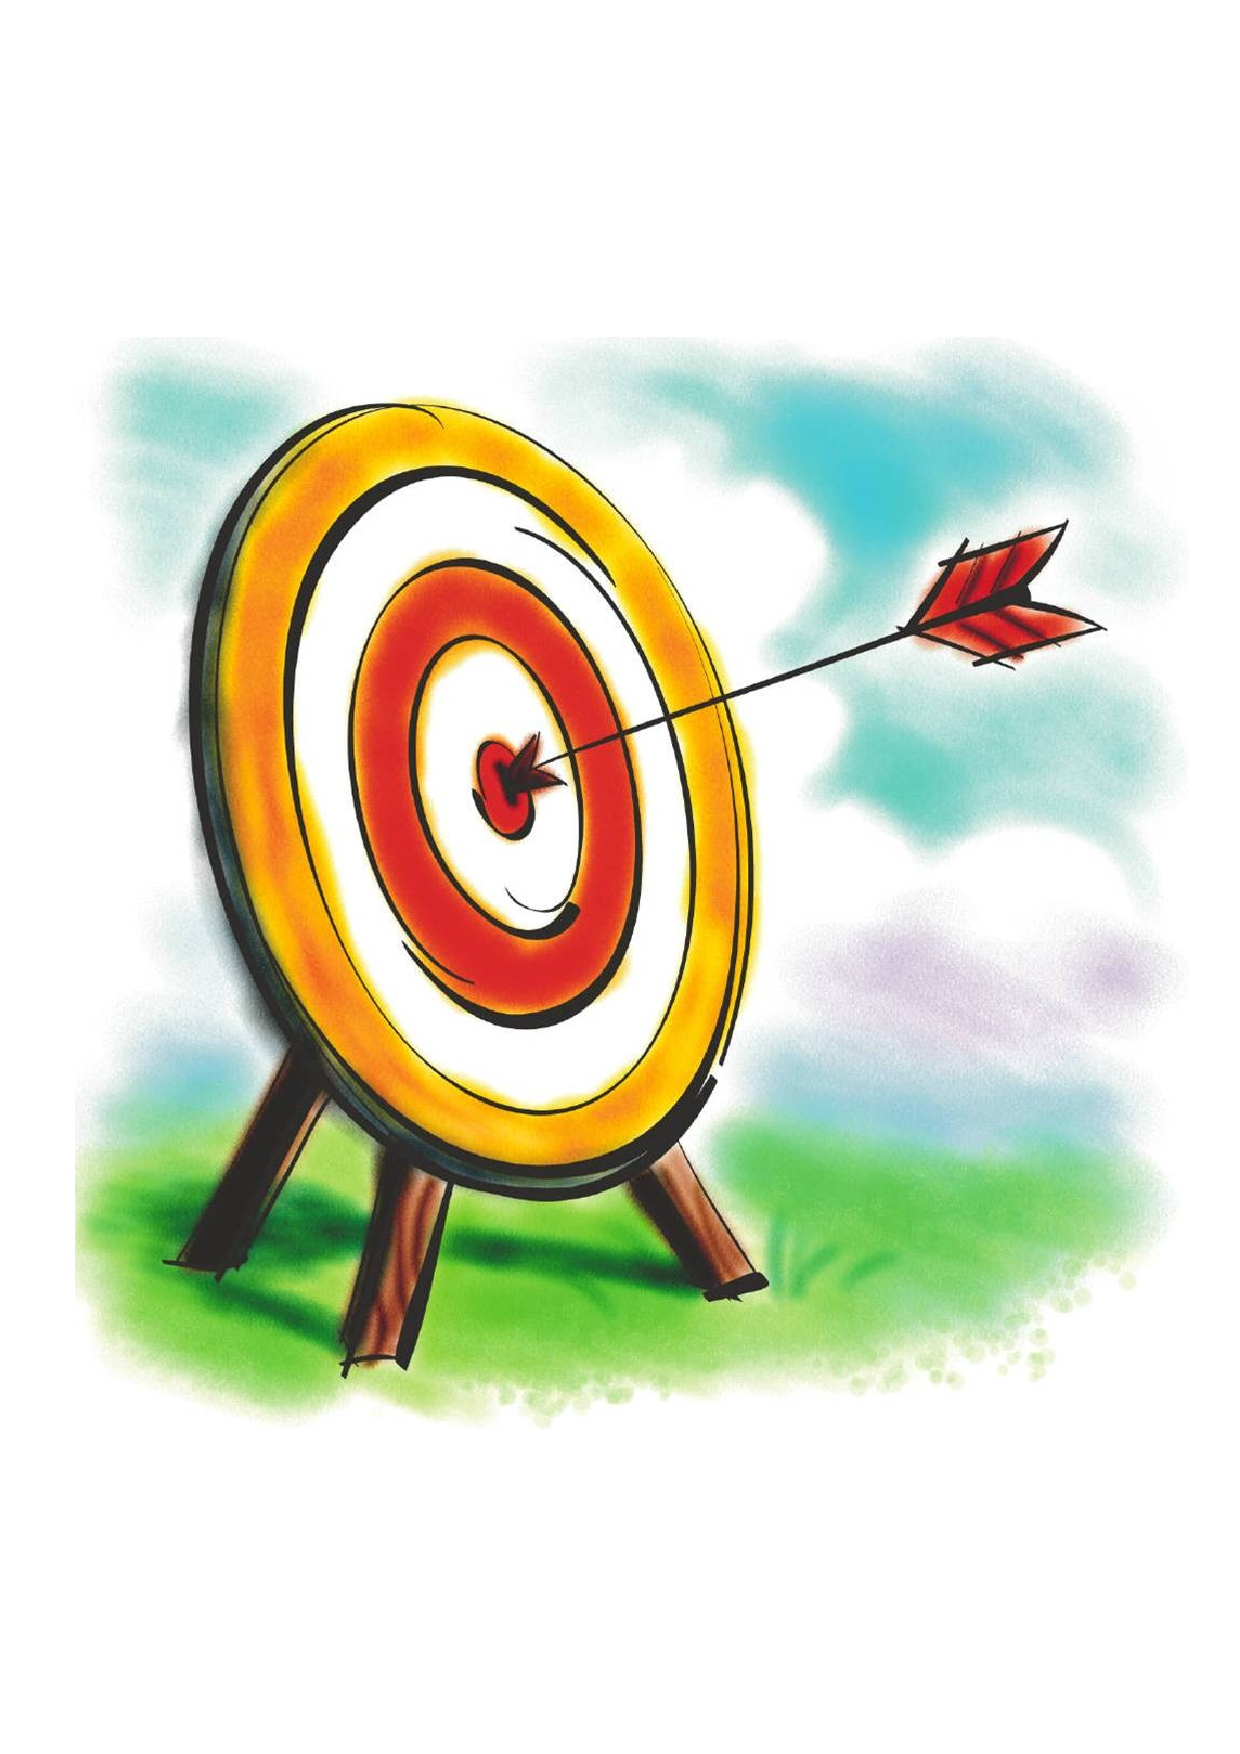
\includegraphics[width=.07\textwidth]{archeryf}}; }
				{\node[fancytitle2,  rounded corners] at (box.west) {\treeBS};}
			}%%
		\end{tikzpicture}
	\end{center}
}%

%%% ============================================================================================

\newcommand{\arcBS}{\noindent\textcolor{red}{\Huge\ding{247}}}
\NewDocumentEnvironment{warning}{g g}{
	\tikzstyle{mybox1} = [draw=red, fill=red!15,very thick, rectangle, rounded corners, inner sep=10pt, inner ysep=20pt]
	\tikzstyle{fancytitle1} =[fill=red!90, text=white]
	\tikzstyle{fancytitle2} =[fill=red!4, text=white]
	\tikzstyle{fancytitle3} =[fill=white, text=white]
	\begin{flushleft}
	\begin{tikzpicture}
	\node [mybox1] (box)\bgroup
	\IfValueTF{#2}{
		\IfFileExists{#2}{\begin{minipage}{.85\textwidth}}{\begin{minipage}{.93\textwidth}}
	}{%%
		\IfFileExists{warining.png}{\begin{minipage}{.85\textwidth}}{\begin{minipage}{.93\textwidth}}
	}%%
	\baselineskip=.95cm
		\begin{RTL}
}{%
		\end{RTL}
	\end{minipage}
	\egroup;
	\IfValueTF{#1}{\node[fancytitle1, left=10pt] at (box.north east) {\hboxR{#1}};}{\node[fancytitle1, left=10pt] at (box.north east) {\hboxR{توجه}};}%
	\IfValueTF{#2}{
		\IfFileExists{#2}
		{\node[fancytitle3, left=3pt,   rounded corners] at (box.west) {\includegraphics[width=.07\textwidth]{#2}}; }
		{\node[fancytitle2,  rounded corners] at (box.west) {\arcBS};}			
	}{%%
		\IfFileExists{warining.png}
		{\node[fancytitle3, left=3pt,   rounded corners] at (box.west) {
\includegraphics[width=.07\textwidth]{warining.png}}; }
		{\node[fancytitle2,  rounded corners] at (box.west) {\arcBS};}
	}%%
	\end{tikzpicture}
	\end{flushleft}
}%

%%% ============================================================================================

\newcommand{\envBS}{\noindent\textcolor{Violet}{\Huge\ding{41}}}
\NewDocumentEnvironment{refer}{g g}{
	\tikzstyle{mybox1} = [draw=Violet, fill=Violet!10,very thick, rectangle, rounded corners, inner sep=10pt, inner ysep=20pt]
	\tikzstyle{fancytitle1} =[fill=Violet!50, text=white]
	\tikzstyle{fancytitle2} =[fill=Violet!20, text=white]
	\tikzstyle{fancytitle3} =[fill=white, text=white]
	\begin{flushleft}
	\begin{tikzpicture}
	\node [mybox1] (box)\bgroup
	\IfValueTF{#2}{
		\IfFileExists{#2}{\begin{minipage}{.85\textwidth}}{\begin{minipage}{.93\textwidth}}
	}{%%
		\IfFileExists{referO.pdf}{\begin{minipage}{.85\textwidth}}{\begin{minipage}{.93\textwidth}}
	}%%
	\baselineskip=.95cm
	\begin{RTL}
}{%
	\end{RTL}
	\end{minipage}
	\egroup;
	\IfValueTF{#1}{\node[fancytitle1, left=10pt] at (box.north east) {\hboxR{#1}};}{\node[fancytitle1, left=10pt] at (box.north east) {\hboxR{مراجع مفید}};}%
	\IfValueTF{#2}{
		\IfFileExists{#2}
		{\node[fancytitle3, left=3pt,   rounded corners] at (box.west) {\includegraphics[width=.07\textwidth]{#2}}; }
		{\node[fancytitle2,  rounded corners] at (box.west) {\envBS};}			
	}{%%
		\IfFileExists{referO.pdf}
		{\node[fancytitle3, left=3pt,   rounded corners] at (box.west) {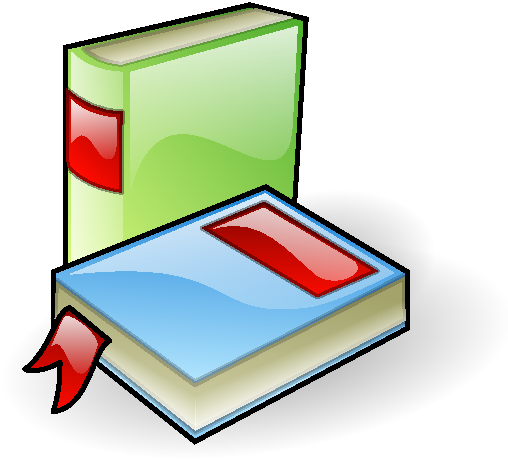
\includegraphics[width=.07\textwidth]{referO}}; }
		{\node[fancytitle2,  rounded corners] at (box.west) {\envBS};}
	}%%
	\end{tikzpicture}
	\end{flushleft}
}%

\newcommand{\goodRef}[1]{ \begin{refer} #1 \end{refer} }

%%% ============================================================================================

\newcommand{\twoBS}{\noindent\textcolor{YellowOrange}{\Huge\ding{44}}}
\NewDocumentEnvironment{info}{g g}{
	\tikzstyle{mybox1} = [draw=YellowOrange, fill=YellowOrange!10,very thick, rectangle, rounded corners, inner sep=10pt, inner ysep=20pt]
	\tikzstyle{fancytitle1} =[fill=YellowOrange!50, text=white]
	\tikzstyle{fancytitle2} =[fill=YellowOrange!15, text=white]
	\tikzstyle{fancytitle3} =[fill=white, text=white]
	\begin{flushleft}
	\begin{tikzpicture}
	\node [mybox1] (box)\bgroup
	\IfValueTF{#2}{
		\IfFileExists{#2}{\begin{minipage}{.85\textwidth}}{\begin{minipage}{.93\textwidth}}
	}{
		\IfFileExists{infoRR.png}{\begin{minipage}{.85\textwidth}}{\begin{minipage}{.93\textwidth}}
	}%%
	\baselineskip=.95cm
	\begin{RTL}
}{%
	\end{RTL}
	\end{minipage}
	\egroup;
	\IfValueTF{#1}{\node[fancytitle1, left=10pt] at (box.north east) {\hboxR{#1}};}{\node[fancytitle1, left=10pt] at (box.north east) {\hboxR{مطالب بیشتر}};}%%
	\IfValueTF{#2}{
		\IfFileExists{#2}
		{\node[fancytitle3, left=3pt,   rounded corners] at (box.west) {\includegraphics[width=.07\textwidth]{#2}}; }
		{\node[fancytitle2,  rounded corners] at (box.west) {\twoBS};}			
	}{
		\IfFileExists{infoRR.png}
		{\node[fancytitle3, left=3pt,   rounded corners] at (box.west) {
\includegraphics[width=.07\textwidth]{infoRR}}; }
		{\node[fancytitle2,  rounded corners] at (box.west) {\twoBS};}
	}%%
	\end{tikzpicture}
	\end{flushleft}
}%

%%% ============================================================================================


\newcommand{\teleBS}{\noindent\textcolor{Mulberry}{\Huge\ding{37}}}
\NewDocumentEnvironment{problem}{g g}{
	\tikzstyle{mybox1} = [draw=Mulberry, fill=Mulberry!10,very thick, rectangle, rounded corners, inner sep=10pt, inner ysep=20pt]
	\tikzstyle{fancytitle1} =[fill=Mulberry!50, text=white]
	\tikzstyle{fancytitle2} =[fill=Mulberry!15, text=white]
	\tikzstyle{fancytitle3} =[fill=white, text=white]
	\begin{flushleft}
	\begin{tikzpicture}
	\node [mybox1] (box)\bgroup
	\IfValueTF{#2}{
		\IfFileExists{#2}{\begin{minipage}{.85\textwidth}}{\begin{minipage}{.93\textwidth}}
	}{
		\IfFileExists{home.png}{\begin{minipage}{.85\textwidth}}{\begin{minipage}{.93\textwidth}}
	}%%
	\baselineskip=\baselineskipVar
	\begin{RTL}
}{%
	\end{RTL}
	\end{minipage}
	\egroup;
	\IfValueTF{#1}{\node[fancytitle1, left=10pt] at (box.north east) {\hboxR{#1}};}{\node[fancytitle1, left=10pt] at (box.north east) {\hboxR{سوال}};}%%
	\IfValueTF{#2}{
		\IfFileExists{#2}
		{\node[fancytitle3, left=3pt,   rounded corners] at (box.west) {\includegraphics[width=.07\textwidth]{#2}}; }
		{\node[fancytitle2,  rounded corners] at (box.west) {\twoBS};}			
	}{
		\IfFileExists{home.png}
		{\node[fancytitle3, left=3pt,   rounded corners] at (box.west) {
\includegraphics[width=.07\textwidth]{home}}; }
		{\node[fancytitle2,  rounded corners] at (box.west) {\teleBS};}
	}%%
	\end{tikzpicture}
	\end{flushleft}
}%


%%% =========================================================================================================

\newcommand{\defBS}{\noindent\textcolor{ForestGreen}{\Huge\ding{45}}}
\NewDocumentEnvironment{mydef}{g g}{
	\tikzstyle{mybox1} = [draw=Plum, fill=Plum!15,very thick, rectangle, rounded corners, inner sep=10pt, inner ysep=20pt]
	\tikzstyle{fancytitle1} =[fill=Plum, text=white]
	\tikzstyle{fancytitle2} =[fill=Plum!5, text=white]
	\tikzstyle{fancytitle3} =[fill=white, text=white]
	\begin{center}
		\begin{tikzpicture}
			\node [mybox1] (box)\bgroup
			\IfValueTF{#2}{
				\IfFileExists{#2}{\begin{minipage}{.85\textwidth}}{\begin{minipage}{.93\textwidth}}
			}{%%
				\IfFileExists{defi.png}{\begin{minipage}{.85\textwidth}}{\begin{minipage}{.93\textwidth}}
			}%%
			\baselineskip=.95cm
				\begin{RTL}
}{%
				\end{RTL}
			\end{minipage}
			\egroup;
			\IfValueTF{#1}{\node[fancytitle1, left=10pt] at (box.north east) {\hboxR{#1}};}{\node[fancytitle1, left=10pt] at (box.north east) {\hboxR{تعریف}};}%
			\IfValueTF{#2}{
				\IfFileExists{#2}
				{\node[fancytitle3, left=3pt,   rounded corners] at (box.west) {\includegraphics[width=.07\textwidth]{#2}}; }
				{\node[fancytitle2,  rounded corners] at (box.west) {\defBS};}			
			}{%%
				\IfFileExists{defi.png}
				{\node[fancytitle3, left=3pt,   rounded corners] at (box.west) {
\includegraphics[width=.07\textwidth]{defi}}; }
				{\node[fancytitle2,  rounded corners] at (box.west) {\defBS};}
			}%%
		\end{tikzpicture}
	\end{center}
}%

%%% =========================================================================================================

\newcommand{\commentBSS}{\noindent\textcolor{ForestGreen}{\Huge\ding{23}}}
\NewDocumentEnvironment{mycomment}{g g}{
	\tikzstyle{mybox1} = [draw=red,fill=none,very thick, rectangle, rounded corners, inner sep=10pt, inner ysep=20pt]
	\tikzstyle{fancytitle1} =[fill=red, text=white]
	\tikzstyle{fancytitle2} =[fill=red!5, text=white]
	\tikzstyle{fancytitle3} =[fill=white, text=white]
	\begin{center}
		\begin{tikzpicture}
			\node [mybox1] (box)\bgroup
			\IfValueTF{#2}{
				\IfFileExists{#2}{\begin{minipage}{.85\textwidth}}{\begin{minipage}{.93\textwidth}}
			}{%%
				\IfFileExists{robah.png}{\begin{minipage}{.85\textwidth}}{\begin{minipage}{.93\textwidth}}
			}%%
			\baselineskip=.95cm
				\begin{RTL}
}{%
				\end{RTL}
			\end{minipage}
			\egroup;
			\IfValueTF{#1}{\node[fancytitle1, left=10pt] at (box.north east) {\hboxR{#1}};}{\node[fancytitle1, left=10pt] at (box.north east) {\hboxR{توضیح}};}%
			\IfValueTF{#2}{
				\IfFileExists{#2}
				{\node[fancytitle3, left=3pt,   rounded corners] at (box.west) {\includegraphics[width=.07\textwidth]{#2}}; }
				{\node[fancytitle2,  rounded corners] at (box.west) {\commentBSS};}			
			}{%%
				\IfFileExists{robah.png}
				{\node[fancytitle3, left=3pt,   rounded corners] at (box.west) {
\includegraphics[width=.07\textwidth]{robah}}; }
				{\node[fancytitle2,  rounded corners] at (box.west) {\commentBSS};}
			}%%
		\end{tikzpicture}
	\end{center}
}%

%%% =========================================================================================================



\newtheoremstyle{ntdefinitionstyle}% name of the style to be used
  {\topsep}% measure of space to leave above the theorem. E.g.: 3pt
  {\topsep}% measure of space to leave below the theorem. E.g.: 3pt
  {}% name of font to use in the body of the theorem
  {0pt}% measure of space to indent
  {\bfseries\color{nttitle}}% name of head font
  {}% punctuation between head and body
  {.5em}% space after theorem head; " " = normal interword space
  {}% Manually specify head  

\newtheoremstyle{nttheoremstyle}% name of the style to be used
  {\topsep}% measure of space to leave above the theorem. E.g.: 3pt
  {\topsep}% measure of space to leave below the theorem. E.g.: 3pt
  {}% name of font to use in the body of the theorem
  {0pt}% measure of space to indent
  {\bfseries\color{nttitle}}% name of head font
  {}% punctuation between head and body
  {.2em}% space after theorem head; " " = normal interword space
  {}% Manually specify head
  
\newtheoremstyle{ntplainstyle}% name of the style to be used
  {\topsep}% measure of space to leave above the theorem. E.g.: 3pt
  {\topsep}% measure of space to leave below the theorem. E.g.: 3pt
  {\itshape}% name of font to use in the body of the theorem
  {0pt}% measure of space to indent
  {\bfseries\color{nttitle}}% name of head font
  {}% punctuation between head and body
  {.5em}% space after theorem head; " " = normal interword space
  {}% Manually specify head  



\definecolor{nttitle}{RGB}{0,177,235}
% رنگ آبی کم‌رنگ پس‌زمینه محیط قضیه و محیط lstlisting
\definecolor{ntback}{RGB}{212,237,255}
% رنگ سبز صفحه عنوان فارسی و انگلیسی کتاب، قسمت‌ها و محیط ntpoint
\definecolor{ntsec}{RGB}{204,233,157}
% رنگ قهوه‌ای محیط تعریف
\definecolor{ntdef}{RGB}{205,0,205}

\definecolor{ntexp}{RGB}{224,110,12}


\mdfdefinestyle{theoremstyle}{%
hidealllines=true,
frametitlerule=false,
innerrightmargin=5pt,
innerleftmargin=5pt,
frametitlerulewidth=0pt,
frametitlefont=\color{white}\large\bfseries,
linewidth=2pt,%
frametitlerule=true,%
frametitlebackgroundcolor=nttitle,
innertopmargin=\topskip,
skipabove=.7\baselineskip,
skipbelow=1.8\baselineskip,
backgroundcolor=nttitle!15,
startinnercode={\baselineskip=.9cm},
startcode={\vspace{.8\topsep}},
splitbottomskip=10pt,
theoremseparator={},
needspace=4\baselineskip
align=center,
}
\mdtheorem[style=theoremstyle]{nttheorem}[theorem]{\hspace*{1pt}قضیه}


\newcounter{ntcounter}
\makeatletter
\renewcommand\thentcounter{\thechapter\@SepMark\arabic{ntcounter}} 
\newenvironment{ntpoint}[1][\empty]{\par\begin{mdframed}[
hidealllines=true,
innertopmargin=9pt,
skipabove=.9\baselineskip,
innermargin=\dimexpr-\marginparwidth-\marginparsep\relax,
innerbottommargin=9pt,
innerrightmargin=5pt,innerleftmargin=5pt,
backgroundcolor=ntsec,
  singleextra={
      \node[
        overlay,
        inner ysep=7pt,
       inner xsep=9pt,
        anchor=east,
       % text width=1.2cm,
       % align=left,
        minimum height=4ex,
        fill=nttitle,
        yshift=-5.2mm,
        xshift=0mm,
        %rounded corners=3pt,
        font=\color{white}\bfseries
      ] at (P) {\rl{نکته~\thentcounter}};
        \draw[white,fill=white] ($(P)-(0pt,1.65mm)$) -- ($(P)-(0pt,8.8mm)$) -- ($(P)-(7pt,5.225mm)$) -- cycle;
      },
   firstextra={
      \node[
       overlay,
        inner ysep=7pt,
       inner xsep=9pt,
        anchor=east,
       % text width=1.2cm,
       % align=left,
        minimum height=4ex,
        fill=nttitle,
        yshift=-5.2mm,
        xshift=0mm,
        %rounded corners=3pt,
        font=\color{white}\bfseries
      ] at (P) {\rl{نکته~\thentcounter}};
        \draw[white,fill=white] ($(P)-(0pt,1.65mm)$) -- ($(P)-(0pt,8.8mm)$) -- ($(P)-(7pt,5.225mm)$) -- cycle;
      },
]\baselineskip=\baselineskipVar\refstepcounter{ntcounter}
\textbf{\ifx\empty#1\hspace*{1.9cm}\relax\else\hspace*{1.65cm}(#1)\fi}%\\[.2cm]%
\noindent\ignorespaces%
\noindent}{\end{mdframed}\par\vspace*{.4ex}}
\@addtoreset{ntcounter}{chapter}
\makeatother


%%%%%%%%%%%%%%%%%%%%%%%%%%%%%%%%%%%%%%%%%%%%%%%%%
% تعریف محیط ntexample


\newcounter{ntexample}
\makeatletter
\renewcommand\thentexample{\thechapter\@SepMark\arabic{ntexample}} 

\newenvironment{ntexample}[1][\empty]{\par\begin{mdframed}[roundcorner=10pt,,align=right,skipabove=.5\baselineskip,
skipbelow=.3\baselineskip,
innertopmargin=10pt,
innerbottommargin=12pt,
usetwoside=false,
innerrightmargin=10pt,
rightmargin=3pt,
innerleftmargin=0pt,
%outermargin=1pt,
%backgroundcolor=brown!25,
 topline=false,bottomline=false,leftline=false,
middlelinewidth=8pt,
%splittopskip=-15pt,
splitbottomskip=5pt,
middlelinecolor=ntexp,
  singleextra={
      \node[
        overlay,
        outer sep=0pt,
        anchor=north west,
        text width=2.1cm,
        minimum height=4ex,
        fill=ntexp,
        yshift=-2mm,
        xshift=-21mm,
        %rounded corners=3pt,
        font=\color{white}\bfseries
      ] at (P) {\rl{مثال~\thentexample}};
      },
   firstextra={
      \node[
        overlay,
        outer sep=0pt,
        anchor=north west,
        text width=2.1cm,
        minimum height=4ex, 
        fill=ntexp,
        yshift=-2mm,
        xshift=-21mm,
        %rounded corners=3pt,
        font=\color{white}\bfseries
      ] at (P) {\rl{مثال~\thentexample}};
      },
]
\baselineskip=\baselineskipVar
\refstepcounter{ntexample}
\hspace*{1.8cm}\textbf{\ifx\empty#1\space\relax\else\space\textcolor{nttitle}{#1}\space \ \fi}%\\[.2cm]%
%\noindent\ignorespaces%
}{\end{mdframed}\par}
\@addtoreset{ntexample}{chapter}
\makeatother


\newenvironment{ntexample2}[1][\empty]{\par\begin{mdframed}[roundcorner=10pt,,align=right,skipabove=.5\baselineskip,
skipbelow=.3\baselineskip,
innertopmargin=10pt,
innerbottommargin=12pt,
usetwoside=false,
innerrightmargin=10pt,
rightmargin=3pt,
innerleftmargin=0pt,
%outermargin=1pt,
%backgroundcolor=brown!25,
 topline=false,bottomline=false,leftline=false,
middlelinewidth=8pt,
%splittopskip=-15pt,
splitbottomskip=5pt,
middlelinecolor=ntexp,
  singleextra={
      \node[
        overlay,
        outer sep=0pt,
        anchor=north west,
        text width=2.1cm,
        minimum height=4ex,
        fill=ntexp,
        yshift=-2mm,
        xshift=-21mm,
        %rounded corners=3pt,
        font=\color{white}\bfseries
      ] at (P) {\rl{مثال}};
      },
   firstextra={
      \node[
        overlay,
        outer sep=0pt,
        anchor=north west,
        text width=2.1cm,
        minimum height=4ex, 
        fill=ntexp,
        yshift=-2mm,
        xshift=-21mm,
        %rounded corners=3pt,
        font=\color{white}\bfseries
      ] at (P) {\rl{مثال}};
      },
]
\baselineskip=\baselineskipVar
\hspace*{1.8cm}\textbf{\ifx\empty#1\space\relax\else\space\textcolor{nttitle}{#1}\space \ \fi}%\\[.2cm]%
%\noindent\ignorespaces%
}{\end{mdframed}\par}
\makeatother

\makeatletter
\newenvironment{ntremember}[1][\empty]{\par\begin{mdframed}[roundcorner=10pt,,align=right,skipabove=.5\baselineskip,
skipbelow=.3\baselineskip,
innertopmargin=10pt,
innerbottommargin=12pt,
usetwoside=false,
innerrightmargin=10pt,
rightmargin=3pt,
innerleftmargin=0pt,
%outermargin=1pt,
%backgroundcolor=brown!25,
 topline=false,bottomline=false,leftline=false,
middlelinewidth=8pt,
%splittopskip=-15pt,
splitbottomskip=5pt,
middlelinecolor=ForestGreen,
  singleextra={
      \node[
        overlay,
        outer sep=0pt,
        anchor=north west,
        text width=2.1cm,
        minimum height=4ex,
        fill=ForestGreen,
        yshift=-2mm,
        xshift=-21mm,
        %rounded corners=3pt,
        font=\color{white}\bfseries
      ] at (P) {\rl{یادآوری}};
      },
   firstextra={
      \node[
        overlay,
        outer sep=0pt,
        anchor=north west,
        text width=2.1cm,
        minimum height=4ex, 
        fill=ForestGreen,
        yshift=-2mm,
        xshift=-21mm,
        %rounded corners=3pt,
        font=\color{white}\bfseries
      ] at (P) {\rl{یادآوری}};
      },
]
\baselineskip=\baselineskipVar
\hspace*{1.8cm}\textbf{\ifx\empty#1\space\relax\else\space\textcolor{nttitle}{#1}\space \ \fi}%\\[.2cm]%
%\noindent\ignorespaces%
}{\end{mdframed}\par}
\makeatother


\newenvironment{ntdefinition}[1][\empty]{\par\begin{mdframed}[roundcorner=10pt,,align=right,skipabove=.5\baselineskip,
skipbelow=.5\baselineskip,
innertopmargin=10pt,
innerbottommargin=0pt,
usetwoside=false,
innerrightmargin=10pt,
rightmargin=3pt,
innerleftmargin=0pt,
%outermargin=1pt,
%backgroundcolor=brown!25,
 topline=false,bottomline=false,leftline=false,
middlelinewidth=8pt,
%splittopskip=-15pt,
splitbottomskip=5pt,
middlelinecolor=ntdef,
  singleextra={
      \node[
        overlay,
        outer sep=0pt,
        anchor=north west,
        text width=2.1cm,
        minimum height=4ex,
        fill=ntdef,
        yshift=-2mm,
        xshift=-21mm,
        %rounded corners=3pt,
        font=\color{white}\bfseries
      ]     at (P) {\rl{تعریف~\thedefinition}};
      },
   firstextra={
      \node[
        overlay,
        outer sep=0pt,
        anchor=north west,
        text width=2.1cm,
        minimum height=4ex, 
        fill=ntdef,
        yshift=-2mm,
        xshift=-21mm,
        %rounded corners=3pt,
        font=\color{white}\bfseries
      ] at (P) {\rl{تعریف~\thedefinition}};
      },
]
\baselineskip=\baselineskipVar
\refstepcounter{definition}
\hspace*{1.8cm}\textbf{\ifx\empty#1\space\relax\else\space\textcolor{nttitle}{#1}\space \ \fi}%
%\noindent\ignorespaces%
}{\end{mdframed}\hspace*{1.5cm} \par}

%%%%%%%%%%%%%%%%%%%%%%%%%%%%%%%%%%%%%%%%%%%%%%%%%
% تعریف محیط ntsolution
\newenvironment{ntsolution}{\par\begin{mdframed}[skipabove=.7\baselineskip,
innertopmargin=0pt,
innerbottommargin=0pt,
innerrightmargin=8pt,innerleftmargin=0pt,
outermargin=-1pt,
%backgroundcolor=green,
 topline=false,bottomline=false,leftline=false,
middlelinewidth=8pt,
middlelinecolor=nttitle,
]
\baselineskip=\baselineskipVar
\textbf{\textcolor{nttitle}{حل}}\ \
\noindent}{\end{mdframed}\par}

%%%%%%%%%%%%%%%%%%%%%%%%%%%%%%%%%%%%%%%%%%%%%%%%%
% تعریف محیط ntproblems برای حروف‌چینی تمرین‌های پایان فصل‌ها
\makeatletter
\newenvironment{ntproblems}[1][تمرین‌ها]{%
\renewcommand{\thesection}{}
\phantomsection\addcontentsline{toc}{section}{\hspace*{2pt}#1}
\vspace*{.7\baselineskip}
\needspace{5\baselineskip}
\begin{fullwidth}
\par
\begin{mdframed}[%outermargin=\dimexpr-\marginparwidth-\marginparsep\relax,align=center,%skipabove=.7\baselineskip,
%skipbelow=.1\baselineskip,
innertopmargin=9pt,
innerbottommargin=9pt,
%outermargin=-5pt,
usetwoside=false,
rightmargin=0pt,
innerrightmargin=5pt,innerleftmargin=0pt,
backgroundcolor=nttitle!15,
topline=false,
bottomline=false,leftline=false,
middlelinewidth=20pt,
middlelinecolor=nttitle,
]
\normalfont\Large\bfseries #1
\end{mdframed}%
\end{fullwidth}
\vspace*{-.5\baselineskip}
\sectionmark{#1}
\renewcommand\theenumi{\color{nttitle}\bfseries\thechapter\@SepMark\arabic{enumi}}
\renewcommand\labelenumi{\theenumi}
\let\p@enumii\@empty
\setlength{\columnsep}{5ex}
\begin{adjmulticols*}{2}{-\dimexpr+\marginparwidth+\marginparsep\relax}{}
\begin{enumerate}[align=left,itemindent=0pt,labelwidth=5ex,leftmargin=6ex
]}
{\end{enumerate}
\raggedcolumns
\end{adjmulticols*}
}  
\makeatother

%%%%%%%%%%%%%%%%%%%%%%%%%%%%%%%%%%%%%%%%%%%%%%%%%
% تعریف محیط ntsolutions برای حروف‌چینی پاسخ تمرین‌ها
\newenvironment{ntsolutions}{%
\setlength{\columnsep}{5ex}
\begin{adjmulticols*}{2}{-\dimexpr+\marginparwidth+\marginparsep\relax}{}
}
{
\raggedcolumns
\end{adjmulticols*}
}  

%%%%%%%%%%%%%%%%%%%%%%%%%%%%%%%%%%%%%%%%%%%%%%%%%
% تعریف دستور ntchsol برای مشخص کردن پاسخ‌های مربوط به هر فصل در محیط ntsolutions
\newcommand{\ntchsol}[1]{
%\vspace*{.7\baselineskip}
%\needspace{4\baselineskip}
\par
\begin{mdframed}[%outermargin=\dimexpr-\marginparwidth-\marginparsep\relax,align=center,
skipabove=.7\baselineskip,
%skipbelow=.1\baselineskip,
innertopmargin=9pt,
innerbottommargin=9pt,
%outermargin=-5pt,
usetwoside=false,
rightmargin=0pt,
innerrightmargin=5pt,innerleftmargin=0pt,
backgroundcolor=nttitle!15,
topline=false,
bottomline=false,leftline=false,
middlelinewidth=20pt,
middlelinecolor=nttitle,
]
\normalfont\Large\bfseries #1
\end{mdframed}%
%\end{fullwidth}
\vspace*{-.5\baselineskip}
}

%%%%%%%%%%%%%%%%%%%%%%%%%%%%%%%%%%%%%%%%%%%%%%%%%

\def\lemmaautorefname{لم}












%%% 0000000000000000000000000000000000000000000000000000000000000000000000000000000000000000000000000000000000000000000000000000000000000000 

%%% تنظیم فاصله خطوط در متن اصلی
\newlength{\baselineskipVar}
\setlength{\baselineskipVar}{1.1cm}

%% تنظیم فاصله خطوط در فهرست‌ها
\newlength{\listlineskipVar}
\setlength{\listlineskipVar}{0.9cm}
%%============================ پاورقی
%% این دستو موجب می‌شود که پاورقی شما به صورت دو ستونه خورده شود.
\twocolumnfootnotes
%% تنظیم‌های مربوط به پاورقی: فاصله پاورقی با متن + فاصله بین خطوط در پاورقی
%\setlength{\footnotesep}{0.6cm}
%\setlength{\skip\footins}{2cm}



%%\part{part}	     				        -1	not in letters
%%\chapter{chapter}		 	                   0	only books and reports
%%\section{section}		 	                   1	not in letters
%%\subsection{subsection}		         2	not in letters
%%\subsubsection{subsubsection}	         3	not in letters
%%\paragraph{paragraph}		                   4	not in letters
%%\subparagraph{subparagraph}	         5	not in letters

%% این دستور تعیین می‌کند که در متن تا چه عمقی شماره‌گذاری انجام شود. 
\setcounter{secnumdepth}{3}

%%% 0000000000000000000000000000000000000000000000000000000000000000000000000000000000000000000000000000000000000000000000000000000000000000
%% باز تعریف محیط شکل

\makeatletter
\renewenvironment{figure}[1][]{
%% تنظیم کننده فاصله بین خطوط در این قسمت
	\baselineskip = .8cm
	 \ifthenelse{\equal{#1}{}}{
		   \@float{figure}
	 }{%%
		   \@float{figure}[#1]
	 }%%
%% این دستور centering در این قسمت موجب می‌شود که عکس شما در وسط متن قرار گیرد. 
	 \centering
}{%
	 \end@float
}%

%% تغییر اندازه فاصله بین خطوط در محیط caption برای figure. برای اضافه کردن این دستور نیاز به وارد کردن بسته caption هست. 
\captionsetup*[figure]{font={stretch=1.7,small}} 

%%% 0000000000000000000000000000000000000000000000000000000000000000000000000000000000000000000000000000000000000000000000000000000000000000 
%%============================ تنظیمات مربوط به فونت و اندازه جداول
%% بازنویسی محیط جدول
\makeatletter
\renewenvironment{table}[1][]{
	\ifthenelse{\equal{#1}{}}{\@float{table}}{\@float{table}[#1]}
	\centering
}{%
	\end@float
}%
\makeatother
	
%% بازنویسی محیط tabular به منظور تنظیم فونت‌های جدول
\let\oldtabular\tabular
\let\endoldtabular\endtabular
\renewenvironment{tabular}{
	\bgroup
	\settextfont[Scale=1.25]{IRNazanin} 
	\setlatintextfont[Scale=1]{Linux Libertine}
	\oldtabular
}{%
	\endoldtabular 
	\egroup
}%

%% تنظیم کننده فاصله بین خطوط (ردیف‌ها) در یک جدول
\renewcommand{\arraystretch}{1.3}
%% تنظیم کننده ضخامت خطوط جدول
%%\renewcommand{\arrayrulewidth}{.55pt}
%% تنظیم فاصله بین خطوط دو خطه (||) و یا (حالت افقی ||)
%%\renewcommand{\doublerulesep}{1pt}

%% تغییر اندازه فاصله بین خطوط در محیط caption برای table. برای اضافه کردن این دستور نیاز به وارد کردن بسته caption هست. 
\captionsetup*[table]{font={stretch=1.7,small}} 

%%% 0000000000000000000000000000000000000000000000000000000000000000000000000000000000000000000000000000000000000000000000000000000000000000

%% باز تعریف محیط document، هر دستوری که می خواهید در ابتدای برنامه اجرا شود را در این قسمت بنویسید.

%% بازنویسی محیط \begin{document}
\let\olddocument\document
\let\endolddocument\enddocument

\makeatletter
\renewenvironment{document}{
	\olddocument
	%% تنظیم استایل سرفصل
	\pagestyle{plain}
	%% تنظیم فاصله بین خطوط با دستور \baselineskip
	\baselineskip = \baselineskipVar
	\pagenumbering{arabic}
}{%
	\endolddocument
}%
\makeatother

%%% 0000000000000000000000000000000000000000000000000000000000000000000000000000000000000000000000000000000000000000000000000000000000000000 


%% محیطی برای قرار دادن abstract در گزارش و یا  در ابتدای هر فصل. در صورت استفاده از این محیط، متون داخل آن با فونتی متفاوت با فونت متن نوشته شده و در ابتدای متن نیز یک کلمه چکیده اضافه می شود. 
\renewenvironment{abstract}{%
	%\section*{چکیده}
	\settextfont[Scale=1.2]{IRNazanin} 
	\setlatintextfont[Scale=1]{Linux Libertine}
}{%
	\clearpage
} % M

%% این دستور تعیین می‌کند که چه تا چه عمقی شماره‌گذاری شود. در خود متن نه در فهرست مطالب دقت کنید که برای تعیین این که در فهرست مطالب تا چه عمقی شماره گذاری صورت بگیرد باید از دستور
%% \setcounter{tocdepth}{....}
%% استفاده کرد که در ادامه می آید. 

\setcounter{tocdepth}{2}
%%  تنظیمات مربوط به فهرست مطالب، بازنویسی محیط فهرست مطالب برای تعیین فاصله خطوط، قرار دادن در bookmark ها
\let\Oldtableofcontents\tableofcontents
\renewcommand{\tableofcontents}{
%% تنظیم کننده فاصله بین خطوط در این قسمت
	\baselineskip = \listlineskipVar
%	\addcontentsline{toc}{chapter}{فهرست مطالب}
	\Oldtableofcontents\clearpage
%% تنظیم کننده فاصله بین خطوط در این قسمت
	\baselineskip = \baselineskipVar
}%

% با این دستور در فهرست مطالب در هنگام آوردن شماره و عنوان فصل در ابتدای آن یک کلمه فصل می گذارد یعنی مثلا می نویسد: (فصل اول: مقدمه ای بر شبکه ..................... ۱)


%%% 0000000000000000000000000000000000000000000000000000000000000000000000000000000000000000000000000000000000000000000000000000000000000000 

%%=========================== تنظمیات محیط فهرست اشکال

%% این دستورات موجب می‌شود که یک تصویر بند انگشتی در فهرست مطالب ظاهر شود. برای این کار می‌بایست در قسمت caption به صورت زیر فایل تصویر نیز وارد شود. 
%% ٍExample: \caption{\lofimage{/Introduction/Person/Shannon} \lr{Claude Shannon}}

\newlength{\lofthumbsize}
\setlength{\lofthumbsize}{2em}

\newif\iflofimage
\DeclareRobustCommand*{\lofimage}[2][]{%
  \iflofimage
    $\vcenter to \lofthumbsize{\vss%
      \hbox to \lofthumbsize{\hss\includegraphics[{width=\lofthumbsize,height=\lofthumbsize,keepaspectratio=true,#1}]{#2}\hss}%
    \vss}$%
    \quad
  \fi
  \ignorespaces
}


%% در دستورات زیر محیط فهرست اشکال باز تعریف شده و اولا این محیط به bookmark اضافه شده و ثانیا مشکل صفحات اضافی حل شده است. ثالثا فاصله خطوط برای زیبایی در این 
%% محیط اندکی کم شده است، ولی دوباره بعد از آوردن این محیط به حالت اولیه برگشته است. در ضمن از شماره گذاری حرفی برای این محیط استفاده شده است. 
\let\Oldlistoffigures\listoffigures
\renewcommand{\listoffigures}{
	\baselineskip = \listlineskipVar
	\cleardoublepage
	\phantomsection
	\addcontentsline{toc}{chapter}{فهرست تصاویر}
	\lofimagetrue
	\Oldlistoffigures\clearpage
	\lofimagefalse
	\baselineskip = \baselineskipVar
}%

%%% 0000000000000000000000000000000000000000000000000000000000000000000000000000000000000000000000000000000000000000000000000000000000000000 

%% در دستورات زیر محیط فهرست جداول باز تعریف شده و اولا این محیط به bookmark اضافه شده و ثانیا مشکل صفحات اضافی حل شده است. ثالثا فاصله خطوط برای زیبایی در این 
%% محیط اندکی کم شده است، ولی دوباره بعد از آوردن این محیط به حالت اولیه برگشته است. در ضمن از شماره گذاری حرفی برای این محیط استفاده شده است. 
\let\Oldlistoftables\listoftables
\renewcommand{\listoftables}{
%% تنظیم کننده فاصله بین خطوط در این قسمت
	\baselineskip = \listlineskipVar
	\cleardoublepage
	\phantomsection
	\addcontentsline{toc}{chapter}{فهرست جداول}
	\Oldlistoftables\clearpage
%% تنظیم کننده فاصله بین خطوط در این قسمت
	\baselineskip = \baselineskipVar
}%

%%% 0000000000000000000000000000000000000000000000000000000000000000000000000000000000000000000000000000000000000000000000000000000000000000 

%% دستورات لازم برای واژه‌نامه‌ها، فهرست اختصارات و فهرست نمادها در  فایل (Gloss) آورده شده است.
%% Data:  2014-07-23
%% xindy -L persian-variant1 -C utf8 -I xindy -M %.xdy -t %.glg -o %.gls %.glo
%% xindy -L persian-variant1 -C utf8 -I xindy -M %.xdy -t %.blg -o %.bls %.blo
%% xindy -L english -C utf8 -I xindy -M %.xdy -t %.alg -o %.acr %.acn
%%% برای اجرا xindy بر روی فایل .tex و تولید واژه‌نامه‌ها و فهرست اختصارات و فهرست نمادها یکسری  فایل تعریف شده است.‌ Latex داده های مربوط به واژه نامه و .. را در این 
%%%  فایل‌ها نگهداری می‌کند. مهم‌ترین option‌ این قسمت این است که 
%%% عنوان واژه‌نامه‌ها و یا فهرست اختصارات و یا فهرست نمادها را می‌توانید در این‌جا مشخص کنید. 
%%% در این جا عباراتی مثل glg، gls، glo و ... پسوند فایل‌هایی است که برای xindy بکار می‌روند. 
 \newglossary[glg]{english}{gls}{glo}{واژه‌نامه انگلیسی به فارسی}
 \newglossary[blg]{persian}{bls}{blo}{واژه‌نامه فارسی به انگلیسی}
 \makeglossaries
 \glsdisablehyper
 
%%% تعریف استایل برای واژه نامه فارسی به انگلیسی، در این استایل واژه‌های فارسی در سمت راست و واژه‌های انگلیسی در سمت چپ خواهند آمد. از حالت گروه ‌بندی استفاده می‌کنیم، 
%%% یعنی واژه‌ها در گروه‌هایی به ترتیب حروف الفبا مرتب می‌شوند، مثلا:
%%% الف
%%% افتصاد ................................... Economy
%%% اشکال ........................................ Failure
%%% ش
%%% شبکه ...................................... Network
\newglossarystyle{myFaToEn}{%
	\renewenvironment{theglossary}{}{}
	\renewcommand*{\glsgroupskip}{\vskip 10mm}
	\renewcommand*{\glsgroupheading}[1]{\subsection*{\glsgetgrouptitle{##1}}}
	\renewcommand*{\glossentry}[2]{\noindent\glsentryname{##1}\dotfill\space \glsentrytext{##1}
		
	}
}

%% % تعریف استایل برای واژه نامه انگلیسی به فارسی، در این استایل واژه‌های فارسی در سمت راست و واژه‌های انگلیسی در سمت چپ خواهند آمد. از حالت گروه ‌بندی استفاده می‌کنیم، 
%% % یعنی واژه‌ها در گروه‌هایی به ترتیب حروف الفبا مرتب می‌شوند، مثلا:
%% % E
%%% Economy ............................... اقتصاد
%% % F
%% % Failure................................... اشکال
%% %N
%% % Network ................................. شبکه

\newglossarystyle{myEntoFa}{%
	%%% این دستور در حقیقت عملیات گروه‌بندی را انجام می‌دهد. بدین صورت که واژه‌ها در بخش‌های جداگانه گروه‌بندی می‌شوند، 
	%%% عنوان بخش همان نام حرفی است که هر واژه در آن گروه با آن شروع شده است. 
	\renewenvironment{theglossary}{}{}
	\renewcommand*{\glsgroupskip}{\vskip 10mm}
	\renewcommand*{\glsgroupheading}[1]{\begin{LTR} \subsection*{\glsgetgrouptitle{##1}} \end{LTR}}
	%%% در این دستور نحوه نمایش واژه‌ها می‌آید. در این جا واژه فارسی در سمت راست و واژه انگلیسی در سمت چپ قرار داده شده است، و بین آن با نقطه پر می‌شود. 
	\renewcommand*{\glossentry}[2]{\noindent\glsentrytext{##1}\dotfill\space \glsentryname{##1}
		
	}
}

%%% تعیین استایل برای فهرست اختصارات
\newglossarystyle{myAbbrlist}{%
	%%% این دستور در حقیقت عملیات گروه‌بندی را انجام می‌دهد. بدین صورت که اختصارات‌ در بخش‌های جداگانه گروه‌بندی می‌شوند، 
	%%% عنوان بخش همان نام حرفی است که هر اختصار در آن گروه با آن شروع شده است. 
	\renewenvironment{theglossary}{}{}
	\renewcommand*{\glsgroupskip}{\vskip 10mm}
	\renewcommand*{\glsgroupheading}[1]{\begin{LTR} \subsection*{\glsgetgrouptitle{##1}} \end{LTR}}
	%%% در این دستور نحوه نمایش اختصارات می‌آید. در این جا حالت کوچک اختصار در سمت چپ و حالت بزرگ در سمت راست قرار داده شده است، و بین آن با نقطه پر می‌شود. 
	\renewcommand*{\glossentry}[2]{\noindent\glsentrytext{##1}\dotfill\space \Glsentrylong{##1}
		
		}
		%%% تغییر نام محیط abbreviation به فهرست اختصارات
	\renewcommand*{\acronymname}{\raggedleft\rl{\textcolor{white}{فهرست اختصارات}}}
}
%%% تعاریف مربوط به تولید واژه نامه و فهرست اختصارات و فهرست نمادها
%%%  در این فایل یکسری دستورات عمومی برای وارد کردن واژه‌نامه آمده است.
%%%  به دلیل این‌که قرار است این دستورات پایه‌ای را بازنویسی کنیم در این‌جا تعریف می‌کنیم. 
\let\oldgls\gls
\let\oldglspl\glspl

\makeatletter

\renewrobustcmd*{\gls}{\@ifstar\@msgls\@mgls}
\newcommand*{\@mgls}[1] {\ifthenelse{\equal{\glsentrytype{#1}}{english}}{\oldgls{#1}\glsuseri{f-#1}}{\lr{\oldgls{#1}}}}
\newcommand*{\@msgls}[1]{\ifthenelse{\equal{\glsentrytype{#1}}{english}}{\glstext{#1}\glsuseri{f-#1}}{\lr{\glsentryname{#1}}\glsuseri{#1}}}

\renewrobustcmd*{\glspl}{\@ifstar\@msglspl\@mglspl}
\newcommand*{\@mglspl}[1] {\ifthenelse{\equal{\glsentrytype{#1}}{english}}{\oldglspl{#1}\glsuseri{f-#1}}{\oldglspl{#1}}}
\newcommand*{\@msglspl}[1]{\ifthenelse{\equal{\glsentrytype{#1}}{english}}{\glsplural{#1}\glsuseri{f-#1}}{\glsentryplural{#1}}\glsuseri{#1}}

\makeatother



\newcommand{\newword}[4]{
	\newglossaryentry{#1}     {type={english},name={\lr{#2}},plural={#4},text={#3},description={}}
	\newglossaryentry{f-#1} {type={persian},name={#3},text={\lr{#2}},description={}}
}

%%% بر طبق این دستور، در اولین باری که واژه مورد نظر از واژه‌نامه وارد شود، پاورقی زده می‌شود. 
\defglsentryfmt[english]{\glsgenentryfmt\ifglsused{\glslabel}{}{\LTRfootnote{\glsentryname{\glslabel}}}}

%%% بر طبق این دستور، در اولین باری که واژه مورد نظر از فهرست اختصارات وارد شود، پاورقی زده می‌شود. 
\defglsentryfmt[acronym]{\glsentryname{\glslabel}\ifglsused{\glslabel}{}{\LTRfootnote{\glsentrydesc{\glslabel}}}}





%%% 0000000000000000000000000000000000000000000000000000000000000000000000000000000000000000000000000000000000000000000000000000000000000000 

%%============================ دستور برای قرار دادن فهرست اختصارات 
\newcommand{\printabbreviation}{
	\cleardoublepage
	\phantomsection
	\baselineskip=.75cm
%% با این دستور عنوان فهرست اختصارات به فهرست مطالب اضافه می‌شود. 
	\addcontentsline{toc}{chapter}{فهرست اختصارات}
	\setglossarystyle{myAbbrlist}
	\begin{LTR}
	\Oldprintglossary[type=acronym]	
	\end{LTR}
	\clearpage
	\baselineskip = \baselineskipVar
}%

\newcommand{\printacronyms}{\printabbreviation}

%%% 0000000000000000000000000000000000000000000000000000000000000000000000000000000000000000000000000000000000000000000000000000000000000000 

%\newcommand{\printnotation}{
%%% تنظیم کننده فاصله بین خطوط در این قسمت
%	\baselineskip = \listlineskipVar
%	\cleardoublepage
%	\phantomsection
%%% با این دستور عنوان فهرست نمادها به فهرست مطالب اضافه می‌شود. 
%	\addcontentsline{toc}{chapter}{فهرست نمادها}
%	\glossarystyle{mylistNotation}
%	\Oldprintglossary[type=symbols]
%	\clearpage
%%% تنظیم کننده فاصله بین خطوط در این قسمت
%	\baselineskip = \baselineskipVar
%}%

%%% 0000000000000000000000000000000000000000000000000000000000000000000000000000000000000000000000000000000000000000000000000000000000000000 

\let\Oldbibliography\bibliography
\RenewDocumentCommand{\bibliography}{g g}{
	\let\appendix\relax
	%% تنظیم کننده فاصله بین خطوط در این قسمت
	\baselineskip=.5cm
%% با این دستور عنوان این قسمت به (مراجع) تغییر پیدا می‌کند. 
	\renewcommand{\bibname}{مراجع}
	\clearpage
	\phantomsection
	\addcontentsline{toc}{chapter}{مراجع}
	\IfValueTF{#2}{
			\bibliographystyle{#2}
			\Oldbibliography{#1}
	}{%%
			\bibliographystyle{ieeetr-fa}
			\Oldbibliography{#1}
	}%%
}%

%%% 0000000000000000000000000000000000000000000000000000000000000000000000000000000000000000000000000000000000000000000000000000000000000000 

%%% در این جا محیط هر دو واژه نامه را باز تعریف کرده ایم، تا اولا مشکل قرار دادن صفحه اضافی را حل کنیم، ثانیا عنوان واژه نامه ها را با دستور addcontentlist وارد فهرست مطالب کرده ایم.
\let\Oldprintglossary\printglossary
\renewcommand{\printglossary}{
	\let\appendix\relax
%% تنظیم کننده فاصله بین خطوط در این قسمت
	\baselineskip=.75cm
	\clearpage
	\phantomsection
%% این دستور موجب این می‌شود که واژه‌نامه‌ها در  حالت دو ستونی نوشته شود. 
	\twocolumn{}
%% با این دستور عنوان واژه‌نامه به فهرست مطالب اضافه می‌شود. 
	\addcontentsline{toc}{chapter}{واژه نامه انگلیسی به فارسی}
	\setglossarystyle{myEntoFa}
	\Oldprintglossary[type=english]
	
	\clearpage
	\phantomsection
%% با این دستور عنوان واژه‌نامه به فهرست مطالب اضافه می‌شود. 
	\addcontentsline{toc}{chapter}{واژه نامه فارسی به انگلیسی}
	\setglossarystyle{myFaToEn}
	\Oldprintglossary[type=persian]
	\onecolumn{}
	\baselineskip = \baselineskipVar
}%


\let\Oldprintindex\printindex
\RenewDocumentCommand{\printindex}{g g}{
	\let\appendix\relax
	%% تنظیم کننده فاصله بین خطوط در این قسمت
	%\baselineskip=.5cm
	%% با این دستور عنوان این قسمت به (مراجع) تغییر پیدا می‌کند. 
	\clearpage
	\phantomsection
	\addcontentsline{toc}{chapter}{نمایه}
	\settextfont[Scale=1.3]{XB Zar} 
	\Oldprintindex
	\defaultFont
}%

%%% 0000000000000000000000000000000000000000000000000000000000000000000000000000000000000000000000000000000000000000000000000000000000000000 

% دستوری برای رنگ‌آمیزی محیط  Item در dinglist
\newcommand{\itemcolor}[1]{\renewcommand{\makelabel}[1]{\color{#1}\hfil ##1}}



\makeatletter
\defpersianfont\chaptertitlefont[Scale=1.6]{B Titr}

\newcommand\mycustomraggedright{%
 \if@RTL\raggedleft%
 \else\raggedright%
 \fi}
\def\@part[#1]#2{%
\ifnum \c@secnumdepth >-2\relax
\refstepcounter{part}%
\addcontentsline{toc}{part}{\thepart\hspace{1em}#1}%
\else
\addcontentsline{toc}{part}{#1}%
\fi
\markboth{}{}%
{\centering
\interlinepenalty \@M
\ifnum \c@secnumdepth >-2\relax
 \huge\bfseries \partname\nobreakspace\thepart
\par
\vskip 20\p@
\fi
\LARGE\bfseries #2\par}%
\@endpart}
\def\@makechapterhead#1{%
  \vspace*{200\p@}%
  {\parindent \z@ \raggedleft \normalfont
    \ifnum \c@secnumdepth >\m@ne
      \if@mainmatter
        \huge\bfseries \@chapapp\space \thechapter
        \par\nobreak
        \vskip 20\p@
      \fi
    \fi
    \interlinepenalty\@M
    \Huge \bfseries \raggedleft{ #1}\par\nobreak
    \vskip 50\p@
  }}

%اگه می‌خواین که کلمه «فصل» رو هم داشته باشین، خط پایین رو غیرفعال کنین.
%\renewcommand{\chaptername}{}
%  نکته جانبی و بی‌ربط به این بحث: اگه می‌خواین که صفحات اول هر فصل، شماره صفحه نداشته باشن، ۹ خط پایین رو فعال کنین.
%\let\origchapter\chapter
%\renewcommand*{\chapter}{% 
%  \fancypagestyle{plain}{%
%    %\fancyhf{}%
%    \renewcommand{\headrulewidth}{0pt}%
%    \renewcommand{\footrulewidth}{0pt}%
%  }%
%\origchapter
%}

\makeatother

%\nouppercaseheads
%\makepagestyle{mystyle}
%\makeevenhead{mystyle}{}{}{\itshape\leftmark\vskip -2mm}
%\makeoddhead{mystyle}{}{}{\itshape\leftmark\vskip -2mm}
%\makeheadrule{mystyle}{ \textwidth }{.8pt}
%\makeevenfoot{mystyle}{}{\thepage}{}
%\makeoddfoot{mystyle}{}{\thepage}{}

%%% این دستور به این خاطر تعریف می‌شود، که اگر بخواهیم مثلا یک کلمه در واژه نامه را Index‌کنیم، مثلا بنویسیم، ‎\index{\glspl{Water}‎}‎، این دستور index درست عمل نمی‌کند. نویسنده بسته glossaries در این باره این طور گفته است.
%%%If you inspect the .idx file you will see that it contains the following:
%%%\indexentry{\glsentryplural{StrictlyStable}|hyperpage}{1}
%%%\index doesn't expand its argument when writing to the .idx file and since xindy doesn't understand (La)TeX commands the index won't be correctly sorted. This is a feature of \index and is not connected with glossaries.
%%%You could try something like
%%%\expandafter\index\expandafter{\glsentryplural{StrictlyStable}}
%%% توسط دستور تعیین شده می‌توان این مشکل را حل کرد. دقت کنید که این دستور می‌بایست حتما برای واژه‌نامه ها فقط تعریف شود.

\let\oldindex\index
\renewcommand{\index}[1]{
\ifthenelse{\equal{\glsentrytype{#1}}{english}}
	{\expandafter\oldindex\expandafter{\glsentrytext{#1}}}
	{ \ifthenelse{\equal{\glsentrytype{#1}}{acronym}}
		{\expandafter\oldindex\expandafter{\glsentrytext{#1}}}
		{\oldindex{#1}}
	}
}





%%%%%%%%%%%%%%%%%%%%%%%%%%%%%%%%%%%%%%%%%%%%%%%%%%%%%%%%%%%%%%%%%%%%%%%%%%%%%%%%%%%%%%%%%%%%%%%%%%%%%%%%%%%%%%%%%%%%%%%%%%%%%%%%%%%%

% begin appendix autoref patch [\autoref subsections in appendix](http://tex.stackexchange.com/questions/149807/autoref-subsections-in-appendix)
% این کد برای حل مشکل appendix قرار داده شده است. هنگامی که در متن از دستور autoref استفاده کنیم و به یک بخش در داخل appendix ارجاع دهیم می نویسد پیوست ۱.۱ نه بخش ۱.۱
\def\appendixautorefname{پیوست}

\makeatletter
\patchcmd{\hyper@makecurrent}{%
    \ifx\Hy@param\Hy@chapterstring
        \let\Hy@param\Hy@chapapp
    \fi
}{%
    \iftoggle{inappendix}{%true-branch
        % list the names of all sectioning counters here
        \@checkappendixparam{chapter}%
        \@checkappendixparam{section}%
        \@checkappendixparam{subsection}%
        \@checkappendixparam{subsubsection}%
        \@checkappendixparam{paragraph}%
        \@checkappendixparam{subparagraph}%
    }{}%
}{}{\errmessage{failed to patch}}

\newcommand*{\@checkappendixparam}[1]{%
    \def\@checkappendixparamtmp{#1}%
    \ifx\Hy@param\@checkappendixparamtmp
        \let\Hy@param\Hy@appendixstring
    \fi
}
\makeatletter

\newtoggle{inappendix}
\togglefalse{inappendix}

\apptocmd{\appendix}{\toggletrue{inappendix}}{}{\errmessage{failed to patch}}
% end appendix autoref patch


%%%%%%%%%%%%%%%%%%%%%%%%%%%%%%%%%%%%%%%%%%%%%%%%%%%%%%%%%%%%%%%%%%%%%%%%%%%%%%%%%%%%%%%%%%%%%%%%%%%%%%%%%%%%%%%%%%%%%%%%%%%%%%%%%%%%




%مخزن واژه‌نامه‌ها و اختصارات
\newword{Abstraction}{Abstraction}
{انتزاع}{}

\newword{Abstract}{Abstract}
{انتزاعی}{}

\newword{AbsoluteMinimum}{Absolute Minimum}
{کمینه مطلق}{}


\newword{AcceptableCell}{Acceptable Cell}
{سلول پذیرفتنی}{سلول‌های پذیرفتنی}

\newword{AccessBurst}{Access Burst}
{توده دسترسی}{توده‌های دسترسی}


%%% S
\newword{Sample}{Sample}
{نمونه}{نمونه‌ها}

\newword{SamplePath}{Sample Path}
{نمونه مسیر}{}

\newword{SampleSpace}{Sample Space}
{فضای نمونه}{فضای نمونه‌ها}
\newacronym{ACK}{ACK}{Acknowledgement}

\newacronym{ACI}{ACI}{Application Control Interface}

\newacronym{ACIR}{ACIR}{Adjacent Channel Interference Ratio}

\newacronym{ACLC}{ACLC}{Adaptive Configuration of Logical Channels}

\newacronym{ACLP}{ACLP}{Adjacent Channel Leakage Power}

\title{
بررسی و ارزیابی حفظ حریم زمانی  در شبکه‌های ارتباطی با استفاده از تئوری صف
}
\supervisor{دکتر احمد خونساری}
\institute{دانشگاه تهران}
\faculity{پرديس دانشکده های فنی}
\group{دانشکده مهندسی برق و کامپيوتر}
\forwhat{رساله برای دریافت درجه دکترای تخصصی}
\field{در رشته مهندسی کامپیوتر گرایش نرم‌افزار}
\author{ابوالفضل دیانت}
\date{دی‌ماه 1395}

\begin{document}
\setlength{\belowdisplayskip}{2pt} \setlength{\belowdisplayshortskip}{2pt}
\setlength{\abovedisplayskip}{2pt} \setlength{\abovedisplayshortskip}{2pt}
\pagenumbering{gobble}
\thesisStyleOO{./Pic/logo}{./Pic/logo2}
\mbox{}\newpage
\Godpage
\mbox{}\newpage
\clearpage\newpage
\begin{table}
\begin{tabular}{ccc}

\includegraphics[width=.15\textwidth]{Pic/logo}&
\begin{minipage}{0.55\linewidth}
\vskip 0.9cm
\begin{center}\Large
\typefontR{\Large
دانشگاه تهران 
}
 \\* [0.5cm]
پرديس دانشکده های فنی\\ [0.5cm]
\end{center}
\end{minipage}
&

\includegraphics[width=.15\textwidth]{Pic/logo2}
\end{tabular}
\end{table}
\begin{center}
\vskip 1.5cm
رساله برای دریافت درجه‌ی دکتری تخصصی در رشته مهندسی  کامپیوتر گرایش نرم‌افزار

\vskip 5pt \textbf{عنوان:}
بررسی و ارزیابی حفظ حریم‌زمانی در شبکه‌های ارتباطی با استفاده از تئوری صف

\vskip 5pt \textbf{نگارش:} 
ابوالفضل دیانت

\end{center}
\vskip 0.9cm\indent
این پایان‌نامه در تاریخ 1395/11/20 در مقابل هیات داوران دفاع گردید و مورد تصویب قرار گرفت. 
\vskip 0.9cm
\vskip 5pt \textbf{
رییس دانشکده‌ی مهندسی برق و کامپیوتر:} دکتر مجید نیلی احمدآبادی

\vskip 5pt \textbf{
معاون پژوهشی و تحصیلات تکمیلی دانشکده مهندسی برق و کامپیوتر:} دکتر بابک نجار اعرابی

\vskip 5pt \textbf{
استاد راهنما:} دکتر احمد خونساری

\vskip 5pt \textbf{
عضو هیات داوران:} دکتر بابک خلج

\vskip 5pt \textbf{
عضو هیات داوران:} دکتر فرید آشتیانی

\vskip 5pt \textbf{
عضو هیات داوران:} دکتر مهدی کارگهی

\vskip 5pt \textbf{
عضو هیات داوران:} دکتر بهنام بهرک

%\vskip 5pt \textbf{
%عضو هیات داوران:} دکتر .... 





















\clearpage
\clearpage\newpage
\makeatletter

\begin{center}
{\LARGE{\textbf{تأییدیه صحت و اصالت نتایج}}}\\*[1cm]
باسمه تعالی
\end{center}


این‌جانب
\textbf{\@author}
به شماره دانشجویی
\textbf{\@authorCode}
دانشجو رشته \textbf{مهندسی کامپیوتر} گرایش \textbf{شبکه‌های کامپیوتری} مقطع تحصیلی \textbf{کارشناسی ارشد }تایید می‌نمایم که کلیه مندرجات در این پایان‌نامه حاصل کار پژوهشی اینجانب تحت نظارت و راهنمایی عضو هیأت علمی دانشگاه علم و صنعت ایران، بدون هرگونه دخل و تصرف انجام گرفته و موارد نسخه‌برداری شده از آثار دیگران، مطابق مقررات و ضوابط ارجاع داده شده و ویژگی‌های کامل منابع را در فهرست منابع ذکر کرده‌ام. این پایان‌نامه پیش‌تر برای احراز هیچ مدرکی ارائه نگردیده است. 

در صورت اثبات خلاف مندرجات فوق، به تشخیص دانشگاه مطابق با ضوابط و مقررات حاکم (قانون حمایت از حقوق مولفان و منصفان و قانون ترجمه، تکثیر و نشریات و آثار صوتی، ضوابط و مقررات آموزشی و پژوهشی، انضباطی و غیره) با اینجانب رفتار خواهد شد و حق هرگونه اعتراض در خصوص احقاق حقوق مکتسب و تشخیص و تعیین تخلف و مجازات را از خویش سلب می‌نمایم. در ضمن، مسئولیت هرگونه پاسخگویی به اشخاص اعم از حقیقی و حقوقی و مراجع ذی‌صلاح (اعم از اداری و قضایی) به عهده اینجانب خواهد بود و دانشگاه هیچ گونه مسئولیتی در این خصوص نخواهد داشت. 

کلیه نتایج و حقوق حاصل از این پایان‌نامه متعلق به دانشگاه علم و صنعت ایران است. هرگونه استفاده از نتایج علمی و عملی و واگذاری اطلاعات به دیگران یا چاپ و تکثیر، نسخه‌برداری، ترجمه و اقتباس از این پایان‌نامه بدون موافقت کتبی دانشگاه علم و صنعت ایران ممنوع است. نقل مطالب با ذکر منبع بلامانع است. 


\vskip 1cm
\begin{flushleft}
\begin{table}[H]
\raggedright
\begin{tabular}{rr}
نام و نام‌خانوادگی دانشجو: &
\@author \\*[5mm]
تاریخ: &
\@date \\*[5mm]
امضای دانشجو: &
\\
\end{tabular}
\end{table}
\end{flushleft}
\makeatother

\newpage
\vspace{4cm}

{\nastaliq
	{\Huge
		تقدیم به همه آنهایی که 
		\vspace{1.5cm}
		
		\hspace{3cm}
		می خواهند بیشتر بدانند
}}


\newpage
{\nastaliq\LARGE
سپاس‌گزاری...
}
\\[2cm]
 ماحصل آموخته هایم را تقدیم می‌کنم به آنان که مهر آسمانی‌شان آرام بخش آلام زمینی ام است.
 
به استوارترین تکیه گاهم،دستان پرمهر پدرم...

به سبزترین نگاه زندگیم،چشمان سبز مادرم...

که هرچه آموختم در مکتب عشق شما آموختم و هرچه بکوشم قطره ای از دریای بی کران مهربانی‌تان را سپاس نتوانم بگویم.

امروز هستی ام به امید شماست و فردا کلید باغ بهشتم رضای شما...

ره‌آوردی گران سنگ تر از این ارزان نداشتم تا به خاک پایتان نثار کنم؛ باشد که حاصل تلاشم نسیم گونه غبار خستگی‌تان را بزداید. بوسه بر دستان پرمهرتان.

هم‌چنین بر خود واجب می‌دانم از زحمات استاد راهنمای خود، جناب آقای دکتر ..... صمیمانه تشکر و  قدردانی کنم  که قطعاً بدون راهنمایی‌های‌ ایشان، این کار به انجام نمی‌رسید. 

\clearpage\newpage
 
{\nastaliq \LARGE
خدایا...%
}\\
\vspace{.5cm}\\
به من زیستنی عطا کن که در لحظه مرگ، بر بی‌ثمری لحظه‌ای که برای زیستن گذشته است، حسرت نخورم   و مُردنی عطا کن که بر بیهودگیش، سوگوار نباشم. بگذار تا آن را، خود انتخاب کنم، اما آنچنان که تو دوست می‌داری.

تو می‌دانی و همه می‌دانند که شکنجه دیدن بخاطر تو، زندانی کشیدن بخاطر تو و رنج بردن به پای تو تنها لذت بزرگ زندگی من است، از شادی توست که من در دل می‌خندم، از امید رهایی توست که برق امید در چشمان خسته‌ام می‌درخشد و از خوشبختی توست که هوای پاک سعادت را در ریه‌هایم احساس می‌کنم. نمی‌توانم خوب حرف بزنم. نیروی شگفتی را که در زیر کلمات ساده و جمله‌های ضعیف و افتاده، پنهان کرده‌ام دریاب، دریاب.

تو می‌دانی و همه می‌دانند که زندگی از تحمیل لبخندی بر لبان من، از آوردن برق امیدی در نگاه من، از برانگیختن موج شعفی در دل من، عاجز است.

تو، چگونه زیستن را به من بیاموز، چگونه مردن را خود خواهم آموخت.

به من توفیق تلاش در شکست، صبر در نومیدی، رفتن بی‌همراه، جهاد بی‌سلاح، کار بی‌پاداش، فداکاری در سکوت، دین بی‌دنیا، مذهب بی‌عوام، عظمت بی‌نام، خدمت بی‌نان، ایمان بی‌ریا، خوبی بی‌نمود، گستاخی بی‌خامی، قناعت بی‌غرور، عشق بی‌هوس، تنهایی در انبوه جمعیت، و دوست داشتن بی‌آنکه دوست بداند،  روزی کن
\RTLfootnote{مناجاتی از دکتر علی شریعتی.}.

\clearpage
\clearpage\newpage
\section*{چکیده}
\baselineskip=.90cm
امروزه نشان داده شده که حتی در صورت استفاده از سازوکارهای تامین امنیت محتوای داده، نظیر رمزنگاری داده‌ها، یک مهاجم باهوش می‌تواند اطلاعات مفیدی را با تحلیل رفتار تولید داده‌ها، بدست آورد. این بدان علت است   که با استفاده از سازوکارهای سنتی رمزنگاری، حریم‌خصوصی بسیاری از جنبه‌های تولید داده نظیر میانگین و پراش زمان تولید داده‌ها،  در برابر یک مهاجم باهوش قابل حفظ نخواهد بود. بدین‌سان علاوه بر استفاده از سازکارهای تامین امنیت محتوای داده و به عنوان مکمل آن، نیاز به ارایه راه کارهایی به منظور حفظ حریم خصوصی این جوانب نیز وجود دارد. به عبارت‌بهتر و از دیدگاه علم
\glspl*{ComputerNetwork}، \gls*{Adversary}
بدون داشتن اطلاعاتی در مورد 
\gls*{ApplicationLayer} و \gls*{TransportLayer}،
و فقط با داشتن اطلاعات زمانی ارسال 
\glspl*{Packet} در \gls*{NetworkLayer}، \gls*{Privacy} \gls*{User}
را به خطر بیاندازد. 

در این رساله، با استفاده از 
‎\gls*{QueuingTheory}‎ و \gls*{InformationTheory}
این جنبه از
\gls*{Privacy}
را مورد بررسی قرار خواهیم داد. ما در ابتدا به سراغ نرخ تولید داده در \gls*{SourceNode} می‌رویم. خواهیم گفت که یک
\gls*{Adversary}
باهوش می‌تواند با بهره‌گرفتن از
\gls*{FlowConservationLaw} و با استفاده از \gls*{Rate}، \gls*{TemporalAndStatisticalPrivacy} \gls*{User}
را به خطر بیاندازد. البته در ادامه خود را محدود به 
\gls*{Rate}
نخواهیم کرد و از یک
\gls*{Feature}
به صورت کلی سخن به میان خواهد آمد. برای
\gls*{Feature} \gls*{Rate}
راه‌کاری نیز مبتنی بر اضافه نمودن
\glspl*{DummyPacket}
ارایه می‌گردد. در ضمن گذری نیز بر 
\gls*{TemporalAndStatisticalPrivacy} در \glspl*{CachingSystem}
خواهیم داشت.
\gls*{Adversary} 
باشنود کانال در مرحله
\gls*{Delivery} در \glspl*{CachingSystem}،
می‌تواند 
\gls*{Privacy} \glspl*{User}
را به خطر بیاندازد، بدین‌سان که می‌تواند دریابد که با احتمال زیادی یک
\gls*{User}،
چه فایلی را درخواست کرده‌است. 

روش‌های پیشنهادی در کل این رساله، می‌بایست به نحوی باشد که  ضمن حفظ
\gls*{TemporalAndStatisticalPrivacy}، ‎\gls*{QoS}‎ \gls*{User}
را نیز حفظ نماید. تمامی روش‌های پیشنهادی ارایه شده در این رساله، بر پایه تعدادی
\gls*{OptimizationProblem}،
استوار است که 
\gls*{TradeOff} بین \gls*{Privacy} و \gls*{Cost}
را مدیریت می‌نماید. از سوی دیگر به منظور مدل‌سازی هرچه بهتر مفهوم
\gls*{Privacy}، 
به سراغ یافتن یک‌سری
\gls*{LowerBound} برای \gls*{AdversarysBestEstimationErrorProbability}
خواهیم رفت. در این راه از باندهای پیشنهاد شده در مبحث 
\glspl*{CommunicationChannel} که در علم \gls*{InformationTheory}
مورد بحث قرار می‌گیرد، استفاده کرده‌ایم.
در نهایت نیز یک مدل ریاضیاتی برای
\glspl*{CachingSystem}
و بالابردن
\gls*{Privacy}
در این نوع از سامانه‌ها با درنظر گرفتن میزان ترافیک مبادله شده پیشنهاد خواهیم داد. 

\textbf{کلمات کلیدی:}
\glsentrytext{Privacy} \glsentrytext{ContextOriented}، 
\glsentrytext{DummyPacket}، 
\glsentrytext{AdversarysBestEstimationErrorProbability}، 
\glsentrytext{InformationTheory}، 
\glsentrytext{CachingSystem}.





\pagenumbering{alph}
\tableofcontents
\listoffigures
\listoftables
\clearpage
\printabbreviation
\pagenumbering{arabic}

\chapter{مقدمه}
\label{chap:introduction}
\begin{abstract}
در این فصل  انگیزه‌ و هدفمان را، در انتخاب موضوع این رساله بیان خواهیم کرد. بدین‌منظور  نخست در
\autoref{sec:introSecTem}
به سراغ مفهوم \gls{Security} خواهیم رفت. خواهیم گفت که امروزه،
\gls{Privacy} \gls{ContextOriented}
اهمیت بی‌بدیلی در حوزه \gls{Security} یافته است. از دریای بی‌کران موضوعات مربوط به 
\gls{Privacy} \gls{ContextOriented}،
به سراغ  مبحث
 ‎\gls{TemporalAndStatisticalPrivacy} ‎ 
خواهیم رفت. برای جلب توجه خواننده به اهمیت موضوع در 
\autoref{sec:IntroApplications}،
برخی از کاربردهای مطرح در این حوزه مورد بررسی قرار خواهد گرفت. در نهایت در 
\autoref{sec:contributionIntr} و \autoref{sec:structureResale}
به ترتیب دستاوردهای حاصل گشته و ساختار رساله ارایه می‌گردد. 
\end{abstract}

\section{از \glsentrytext{Security} تا \glsentrytext{TemporalAndStatisticalPrivacy}}
\label{sec:introSecTem} \index{\glsentrytext{Security}}
\gls{Security}
از مهم‌ترین واژه‌هایی است که در فکر و ذهن بشر، از نخستین لحظات زندگانی‌اش در جریان بوده‌است. هنگامی که  ژولیوس سزار‎‎\LTRfootnote{Gaius Iulius Caesar}‎
برای نخستین بار در ۵۰ سال قبل از میلاد، رمز ساده جانشینی حرفی خود را بکار گرفت، هیچ‌گاه فکر نمی‌کرد که حوزه‌ای که در آن گام نهاده، به یکی از بزرگترین حوزه‌های تحقیقاتی دنیا مبدل خواهد شد. 
\gls{Security}
در حوالی جنگ جهانی دوم رشد شگرفی را تجربه کرد. اما آن‌چه که ما اکنون بر  آن گام می‌نهیم، مدیون دو انقلاب  بزرگ در این حوزه است، مقاله ۱۹۴۹ شانون\LTRfootnote{
Claude Elwood Shannon (April 30, 1916 – Feb 24, 2001)} \cite{Shannon1949Communication}
 و دیگری بوجود آمدن مفهوم امنیت مبتنی بر 
\gls{PublicKey} \cite{menezes1996handbook}.

تا مدت‌ها نگاه ما به 
\gls{Security}
به سه‌گانه
\gls{CIA}
خلاصه می‌گشت، اما با گذر زمان مفاهیم جدیدی نظیر
\gls{Freshness}, \gls{Nonrepudiation}, \gls{Anonymity} و \gls{Privacy}
نیز مطرح گشت و جای خود را در این حوزه پیدا کرد
\cite{menezes1996handbook}.
در این مجال، از دریای بی‌کران
\gls{Security}، به سراغ \gls{Privacy}
می‌رویم. 

\index{\glsentrytext{Privacy}}
\index{\glsentrytext{Privacy}!\glsentrytext{DataOriented}}
\index{\glsentrytext{Privacy}!\glsentrytext{ContextOriented}}
\gls{Privacy}
را می‌توان در دو دسته
\gls{DataOriented} و \gls{ContextOriented}
طبقه‌بندی نمود
\cite[بخش $12.4.1$]{guizani2015future}, \cite[صفحه 202]{mason2014sensing}.
نقطه تمرکز 
\gls{Privacy} \gls{DataOriented}،
بر روی محتوای داده است و بدین‌سان سازوکارهایی نظیر 
\gls{Encryption}, \gls{Integrity} و غیره
برای تامین چنین نیازی کارا و کافی خواهد بود. اما در این رساله به سراغ دسته دوم یعنی
\gls{Privacy} \gls{ContextOriented} 
می‌رویم.  در این دسته بالعکس دسته نخست، هدف غایی کسب اطلاعات جانبی  از داده‌ها است. فرض کنید جلسه‌ای محرمانه بین دو نفر تشکیل شده است. در این نوع از 
\gls{Privacy}،
محتوای داده (صحبت‌هایی که در جلسه مطرح شده) برای ما اهمیت ندارد، بلکه اطلاعات جانبی آن نظیر  این‌که چه‌کسانی، درکجا، کی، چگونه و چرا این جلسه را برگزار کردند، از اهمیت بیشتری برخوردار خواهد بود. 

\index{\glsentrytext{TemporalAndStatisticalPrivacy}!مفهوم}
آن‌چه که ما در این رساله به دنبال آن هستیم، نوعی از 
\gls{Privacy} \gls{ContextOriented} 
است، که ما آن را
\gls{TemporalAndStatisticalPrivacy}
می‌نامیم. در
\autoref{fig:WhatInThesis}
نسبت موضوع انتخاب گشته (یعنی 
\gls{TemporalAndStatisticalPrivacy}) 
به نسبت کل حوزه
\gls{Security}
به خوبی نشان داده شده است. خواهید دید که در
\gls{TemporalAndStatisticalPrivacy}،
 هر نوع اطلاعاتی از زمان رخداد یک حادثه چه به صورت قطعی و چه به صورت آماری (به عنوان نمونه نرخ و \gls{Variance} زمان رخداد آن حادثه) 
ممکن است 
\gls{Privacy} \gls{User}
را به مخاطره بیافکند. در ادامه برخی از کاربردهای این نوع از 
\gls{Privacy}
را ذکر خواهیم کرد.
\begin{figure}
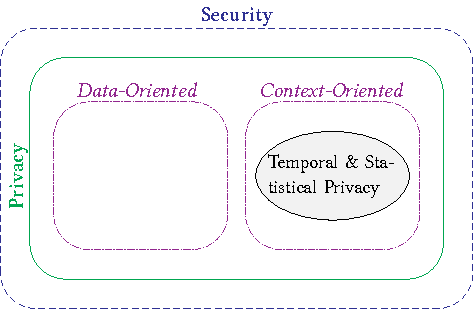
\includegraphics[width=0.6\linewidth]{Pic/WhatInThesis/mainFig}
\caption{\lofimage{Pic/WhatInThesis/mainFig}
حفظ
\gls*{Privacy}،
یکی از مهم‌ترین ابعاد حفظ
\gls*{Security} یک \gls*{System}
است. 
\gls*{Privacy} به نوبه خود به دو بخش \gls*{DataOriented} و \gls*{ContextOriented}
تقسیم‌ می‌گردد. در این رساله ما به دنبال پویش در حوزه
\gls*{TemporalAndStatisticalPrivacy} 
(از زیرمجموعه
\gls*{Privacy} \gls*{ContextOriented})
هستیم.
}
\label{fig:WhatInThesis}
\end{figure}



\section{کاربردهای \glsentrytext{TemporalAndStatisticalPrivacy}}
\index{\glsentrytext{TemporalAndStatisticalPrivacy}!کاربرد}
\label{sec:IntroApplications}
\gls*{TemporalAndStatisticalPrivacy}
از جنبه‌های بسیاری می‌تواند حائز اهمیت باشد. در ادامه ما به چند نمونه از این کاربردها اشاره خواهیم نمود. البته کاربردهای مساله یاد شده، به موضوعات مورد اشاره محدود نمی‌شود، و موارد اشاره شده تنها نمونه‌هایی از کاربردهای این حوزه هستند.

\subsection{\glsentrytext{Privacy} \glsentrytext{User} در حوزه \glsentrytext{TrafficClassification}} \index{\glsentrytext{PacketInspection}}
\index{\glsentrytext{TrafficClassification}}
تا چند سال پیش، تقریبا همه  ‎\gls{Application}هایی که بر روی رایانه‌ها اجرا می‌شدند، از پروتکل‌های شناخته شده با ‎\gls{PortNumber}‎ مشخص استفاده می‌کردند؛ به مانند
\gls{Application} \lr{FileZilla}
که از پروتکل
\gls{FTP} و \gls{PortNumber} $20$ و $21$
استفاده می‌کند. اما امروزه تعداد
‎\glspl{Application}‎ی
با پروتکل نامعلوم و اختصاصی، با ‎\gls{PortNumber}‎های غیراستاندارد و تصادفی بسیار فراگیر شده است. به عنوان نمونه‌ای از این 
\glspl{Application}‎
می‌توان از 
\lr{Skype},  \lr{BitTorrent} و \lr{VPN}
نام برد. در ضمن استفاده از سازوکارهای امنیتی در \glspl{Packet}ی تولید شده توسط کاربردهای یاد شده، موجب می‌شود که از محتوای \gls{Packet}، نتوان ‎‎‎‎پی به ‎‎\gls{Application}‎ تولید کننده آن برد. 

یک
\gls{Adversary}
بنا به جهات بسیاری تمایل دارد که دریابد که در 
\gls{SourceNode} چه \gls{Application}ی
اجرا شده است. این موضوع در حوزه‌ای از تحقیقات به نام 
\gls{TrafficClassification}‌ و یا \gls{PacketInspection}
مورد بررسی قرار می‌گیرد. روش‌های مختلفی برای کمک به \gls{Adversary} در این زمینه وجود دارد که دو نمونه از مهم‌ترین این روش‌ها به شرح زیر است
\cite{Valenti2013Reviewing} (\autoref{fig:NetworkLayers}):
\begin{figure}
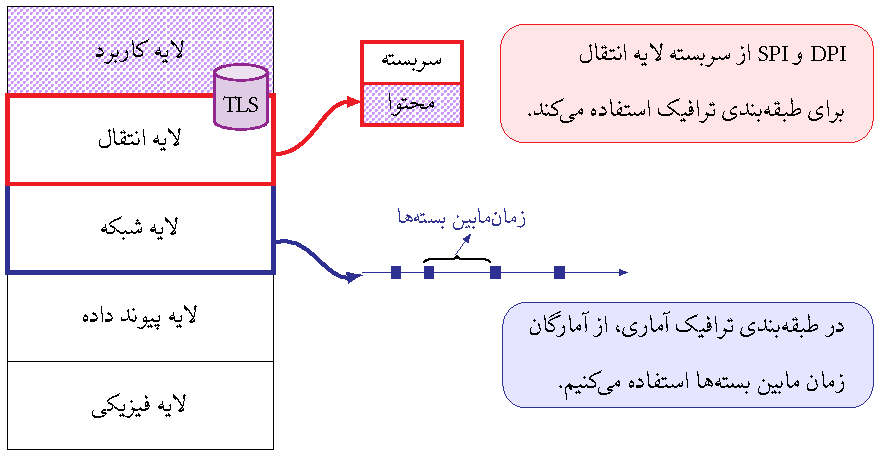
\includegraphics[width=0.75\linewidth]{Pic/NetworkLayers/mainFig}
\caption{\lofimage{Pic/NetworkLayers/mainFig}
در
\gls*{DPI} و \gls*{SPI} از محتوای \gls*{Header} \gls*{TransportLayer}
استفاده می‌شود، در حالی‌که در 
\gls*{TrafficClassification} آماری
 از آمارگان
\gls*{InterDepartureTime} \glspl*{Packet}
استفاده می‌گردد. 
}
\label{fig:NetworkLayers}
\end{figure}
\index{\glsentryname{DPI}}
\index{\glsentryname{SPI}}
\begin{itemize}
\hand \textbf{\gls{TrafficClassification}
بر مبنای ‎\gls{Payload}}‎: در این روش محتوای 
\gls{Header} \gls{TransportLayer}
 مورد بازرسی قرار می‌گیرد. در حالت کلی این روش دسته‌بندی، به دو صورت ‎\gls{DPI}‎‌ و ‎\gls{SPI}‎ انجام می‌پذیرد.
\begin{itemize}
\sci
 در ‎\gls{DPI}‎، سعی می‌شود که ‎\gls{Payload}‎ با یک امضای ثابت مقایسه گردد. دسته‌بندی بر مبنای پروتکل و ‎‎\gls{PortNumber}‎، به عنوان یکی از زیردسته‌های ‎\gls{DPI}‎ ‌محسوب می‌گردد. 
\gls{DPI}
به صورت گسترده در نرم‌افزارها و ‎\glspl{Firewall}‎ مورد استفاده قرار می‌گیرد
\cite{AbuHmed2008Survey}.
\sci

در ‎\gls{SPI}‎، ویژگی‌های آماری ‎
\gls{Header} و \gls{Payload}ی \gls{Packet} \gls{TransportLayer}،
مورد پویش قرار می‌گیرد
\cite{finamore2010kiss}.
\end{itemize}
\index{\glsentrytext{TrafficClassification}!\glsentrytext{Statistical}ی}
\hand \textbf{\gls{TrafficClassification} ‎\gls{Statistical}ی}‎:
 در این شیوه به ویژگی‌های آماری 
\gls{InterDepartureTime} و طول \glspl{Packet} در \gls{NetworkLayer}
توجه می‌شود. لازم به ذکر است که د‎ر دسته‌بندی آماری بر خلاف \gls{SPI} نیازی به بازگشایی
\gls{Packet}
وجود ندارد، بدین‌سان در این نوع از دسته‌بندی‌ حجم پردازش و محاسبات، به مراتب کمتر از 
\gls{SPI}
است. 
\end{itemize}
با زیاد شدن پروتکل‌ها،  مخفی ماندن جزئیات کارکرد آن‌ها به دلایل تجاری و استفاده از سازوکارهای امنیتی نظیر
\lr{IPSec}،
 روش‌های 
\gls{DPI} و \gls{SPI}
دیگر به خوبی نمی‌توانند جواب‌گوی ما در این مساله باشند، و بدین‌سان امروزه شاهد یک اقبال عمومی به روش‌های
\gls{TrafficClassification} ‎\gls{Statistical}ی
هستیم
\cite{Muehlstein2016Analyzing,Crotti2007Traffic}.
پرواضح است که هیچ‌کدام از ما دوست نخواهیم داشت که کسی بداند که چه
\gls{Application}ی
را در هر بازه زمانی بر روی رایانه خود اجرا می‌کنیم. این امر به نوعی جزوی از
\gls{Privacy}
ما محسوب می‌گردد. در این رساله یک چارچوب کلی برای  حفظ 
\gls{Privacy}
در مقابل این نوع از حملات ارایه می‌گردد. 


\subsection{\glsentrytext{TemporalAndStatisticalPrivacy} در \glsentryplural{WirelessSensorNetwork}}
\begin{figure}
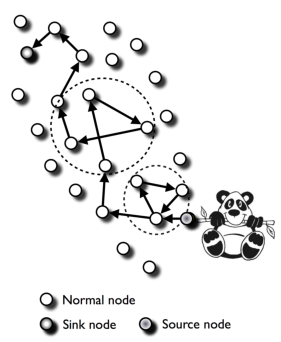
\includegraphics[width=0.45\linewidth]{./Pic/IntroductionPics/panda}
\caption[\lofimage{./Pic/IntroductionPics/panda}
حسگر‌ها به محض حس یک پاندا، گزارشی به صورت ‎\gls*{Multihop}‎ ارسال می‌کنند.]
{حسگر‌ها به محض حس یک پاندا، گزارشی به صورت ‎\gls*{Multihop}‎ ارسال می‌کنند
\cite{conti2013Providing}.}
\label{fig:panda}
\end{figure}
\lr{Ozturk}
در
\cite{Ozturk2004Source}،
مساله‌ای به نام ‎\lr{Panda-Hunter}‎ را معرفی کرده است که برطبق آن تعداد زیادی
\gls{Sensor}،
در منطقه‌ای به منظور تشخیص وجود ‎پانداها قرار داده شده است
(\autoref{fig:panda}).
هر زمان که وجود پاندایی توسط \gls{Sensor} تشخیص داده شود، سیگنالی به مرکز جمع‌آوری داده ارسال می‌گردد. 
\glspl{Sensor}
توسط پروتکل‌های
\gls{Routing} ‎\gls{Multihop}‎، 
داده خود را به دست مرکز جمع‌آوری می‌رسانند. شکارچی نیز وجود دارد که قصد دارد توسط اطلاعات ارسالی از \glspl{Sensor} به محل پاندا پی ببرد. به همین علت شکارچی  به شنود کانال منتهی به مرکز جمع‌آوری مبادرت می‌ورزد.

با رسیدن سیگنال یک \gls{Sensor} به مرکز، شکارچی در می‌یابد که اتفاقی افتاده، و بدین‌سان سعی می‌کند که مکانی که اتفاق مورد نظر رخ داده است را بیابد. از سوی دیگر، شکارچی با بدست آوردن این اطلاعات، می‌تواند نحوه رفتار حرکت پانداها را تخمین بزند، و دریابد که به احتمال زیاد در هر ساعت از شبانه‌روز، پانداها در کدام محل قرار گرفته‌اند. به نظر می‌رسد که در هر دو حالت یاد شده، مبحث ‎\gls{TemporalAndStatisticalPrivacy}‎ از اهمیت ویژه‌ای برخوردار باشد. 

\subsection{\glsentrytext{TemporalAndStatisticalPrivacy} در \glsentrytext{WBAN}}
\begin{figure}
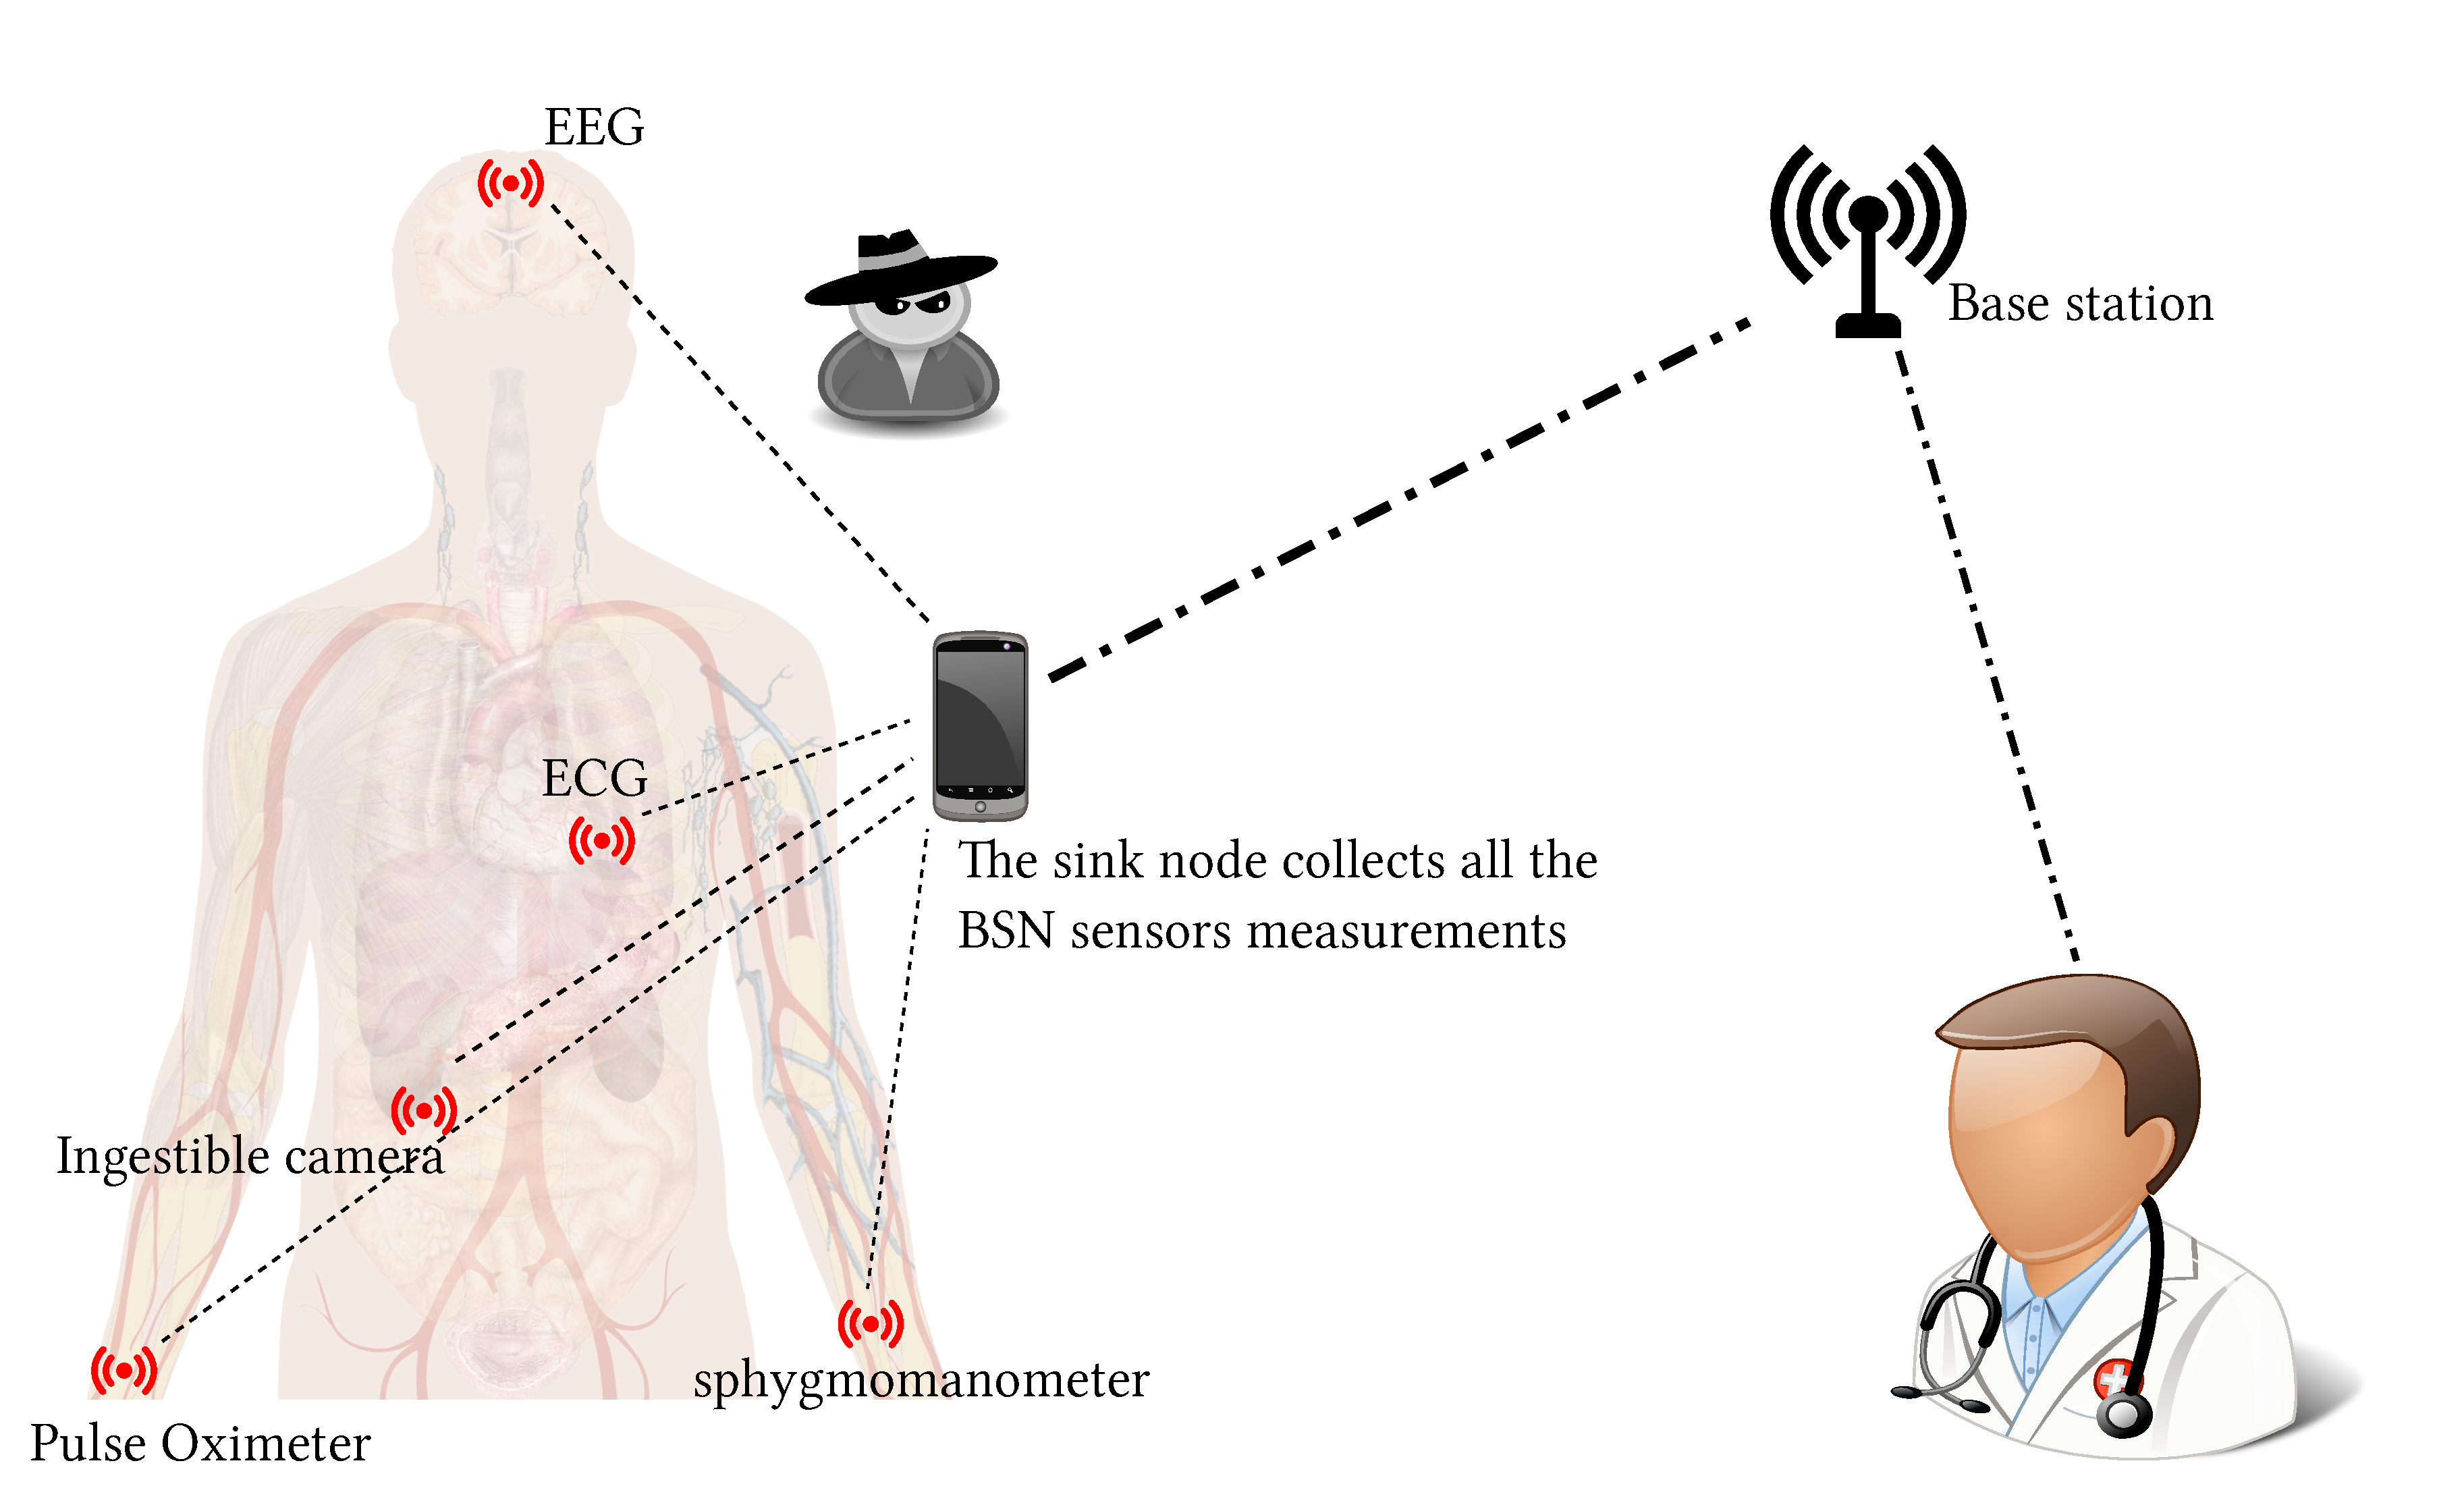
\includegraphics[width=0.7\linewidth]{Pic/IntroductionPics/WBAN}
\caption{\lofimage{Pic/IntroductionPics/WBAN}
\glspl*{Sensor}ی
نصب شده بر روی بدن بیمار در 
\gls*{WBAN}،
در زمان‌های مشخص به اندازه‌گیری علایم حیاتی او می‌پردازد. یک
\gls*{Adversary}
باهوش می‌تواند با بدست‌آوردن اطلاعات مربوط به زمان‌های اندازه‌گیری 
\glspl*{Sensor}،
پی به بیماری فرد ببرد.
}
\label{fig:WBAN}
\end{figure}
در 
\gls{WBAN} تعدادی \gls{Sensor} 
به منظور سنجش ضربان قلب، وضعیت مغز، قند، فشار، چربی و غیره، بر روی بدن بیمار  نصب می‌گردد
\cite{ullah2012comprehensive}.
بسته به نوع بیماری فرد، این 
\glspl{Sensor}
با نرخ‌های مختلفی سنجش‌های مذکور را انجام می‌دهند. به عنوان مثال فرض کنید که مریضی به علت بیماری دیابت در بیمارستان بستری شده است. پرواضح است که برای تنظیم میزان انسولین تزریقی به بیمار، نیاز است در طول روز، حداقل چهار بار میزان قند خون او سنجیده شود، در حالی‌که این تعداد اندازه‌گیری  برای سنجش چربی خون و ضربان قلب نیاز نخواهد بود. در هر بار سنجش،
\gls{Sensor}
سیگنالی را به گره مرکزی ارسال و سپس از آن‌جا این اطلاعات در صورت نیاز به پزشک معالج نیز ارایه می‌گردد.

همان‌طور که در
\autoref{fig:WBAN}
نشان داده شده، فرض کنید که یک
\gls{Adversary}
دستگاهی را در کنار تخت بیمار کار گذاشته است که هنگام ارسال سیگنال توسط هر 
\gls{Sensor}
به گره مرکزی، متوجه ارسال سیگنال می‌گردد. گرچه به علت استفاده از سازوکارهای رمزنگاری، شاید نتواند به میزان سنجه مورد اندازه‌گیری پی ببرد. اما یک
\gls{Adversary}
باهوش می‌تواند با تحلیل اطلاعات مربوط به زمان‌های ارسال سیگنال توسط هر 
\gls{Sensor}،
پی به نوع بیماری فرد ببرد. با کمی دقت می‌توان دریافت که این موضوع، به طور قطع ناقض 
\gls{Privacy}
بیمار است. 


\subsection{تشخیص \glsentrytext{Anomaly}}
فرض کنید که یک
\gls{Malware}
به رایانه شما نفوذ کرده است. نرم‌افزارهایی که برای نابودی
\glspl{Malware}
بکار گرفته می‌شوند، دو ایده کلی را دنبال می‌کنند؛ یا آن‌ها با فعالیت و نحوه تاثیر 
\gls{Malware}
آشنا هستند، و یا در صورت ناآشنا بودن با آن، به رهگیری رفتارهای غیر معمول در  \gls{OperatingSystem} می‌پردازند، و در صورت بروز چنین رفتارهایی، عامل آن رفتار را به عنوان 
\gls{Malware}
تشخیص می‌دهند
\cite{salem2008survey}.
این‌که
\gls{Malware}
به چه قسمتی از رایانه، در چه زمانی و با چه آمارگانی دسترسی پیدا می‌کند، رفتار یک
\gls{Malware}
را تشکیل می‌دهد.

بازهم ادعا می‌کنیم که چارچوب ارایه شده می‌تواند هم به 
\gls{Malware}
و هم به نگهبان رایانه شما یاری رساند. از یک سو چارچوب ارایه شده برای 
\gls{Malware}
می‌تواند مفید باشد چرا که کمک می‌کند تا اطلاعات زمانی و آماری نحوه دسترسی 
\gls{Malware}
مخفی گردد. از سوی دیگر به شما کمک می‌کند تا بتوانید ویژگی‌های زمانی و آماریی از
\gls{Malware}
استخراج نمایید که نسبت به بسیار از اتفاقاتی که در
\gls{OperatingSystem}
رخ می‌دهد، مقاوم باشد. 

\section{نوآوری‌ها}
\label{sec:contributionIntr}
در ادامه به صورت مختصر دستاوردها و نوآوری‌های بدست‌آمده در این رساله را ذکر می‌کنیم. گرچه لازم به ذکر است که هر یک از دستاوردها  متناظر با فصلی از رساله است که در جای خویش به تشریح بیان خواهد شد. 
\begin{itemize}
\sci
در
\autoref{chap:ratePrivacy}،
روشی پیشنهاد خواهیم داد که در آن با استفاده از اضافه کردن تعدادی بسته که ما از آن‌ها با عنوان
 \glspl{DummyPacket}
یاد می‌کنیم، سعی داریم که 
\gls{Privacy} \gls{Rate}
را حفظ کنیم. لازم به ذکر است که در روش پیشنهادی به منظور حفظ
\gls{QoS}،
تنها تعدادی بسته اضافه خواهد گشت و بسته‌ای حذف نخواهد شد. در همان فصل خواهید دید که با استفاده از 
\gls{FanoSInequality} \cite[قضیه $2.10.1$]{cover2006elements}،
معیاری برای توصیف ریاضیاتی
\gls{Privacy}
پیشنهاد خواهیم داد. سپس با یاری‌جستن از یک 
\gls{OptimizationProblem}، \gls{TradeOff} بین \gls{Privacy} و \gls{CommunicationCost}‌ناشی از ارسال
 \glspl{DummyPacket}،
مدیریت خواهد شد. در 
\autoref{sec:contribution}،
به صورت جزئی‌تر به تشریح دستاوردهای حاصل گشته در این قسمت، مبادرت خواهیم ورزید. در ضمن مطالب بیان شده، در مقاله زیر نیز ارایه گشته است. 
\begin{latin}
\baselineskip=.8cm
A. Diyanat, A. Khonsari, and S. P. Shariatpanahi, “A Dummy-Based Approach for Preserving Source Rate Privacy,” \textit{IEEE Transactions on Information Forensics and Security}, vol. 11, no. 6, pp. 1321–1332, Jun. 2016.
\end{latin}
\sci
در
\autoref{chap:FeaturePrivacy}،
توسعه‌ای همه‌جانبه بر مطالب
\autoref{chap:ratePrivacy}
خواهیم داشت. اولا خود را محدود به \gls{Rate} نخواهیم کرد، و به صورت کلی در مورد حفظ 
\gls{Privacy} یک \gls{Feature}
صحبت خواهیم نمود.  ثانیا 
\gls{Mapping}
بین 
\glspl{Feature}
به صورت کلی در نظر گرفته می‌شود؛ به عبارت‌بهتر اگر
\gls{Feature} را همان \gls{Rate}
در نظر بگیریم، هم می‌توان با اضافه کردن
\glspl{DummyPacket}، به \gls{Rate}
اضافه کرد و هم با حذف برخی از 
\glspl{Packet}، از \gls{Rate}
کاست.  در ضمن فرضی نیز بر روی توزیع اجرای 
\glspl{Application}
نخواهیم داشت. از سوی دیگر سه 
\gls{LowerBound} به منظور توصیف \gls{AdversarysBestEstimationErrorProbability}
با بهره‌گیری از علم
\gls{InformationTheory}
بکار گرفته می‌شود. ضمن تشریح نوآوری بدست آمده در این فصل در 
\autoref{sec:contributionExt}،
این مطالب در مقاله زیر نیز ارایه گشته است. 
\begin{latin}
\baselineskip=.8cm
A. H. RezaeiTabar, A. Diyanat, and A. Khonsari, “On the Perfect Privacy: a Statistical Analysis of Network Traffic Approach,” \textit{IEEE Communications Letters}, pp. 1–4, 2016.
\end{latin}
\sci
در 
\autoref{chap:privacyInCaching}،
به سراغ 
\glspl{CachingSystem}
خواهیم رفت. در آن‌جا ذکر خواهد شد که اگر یک
\gls{Adversary}
باهوش، به شنود 
\gls{Link}
ارتباطی بین
\gls{AP} تا \gls{Server}
بپردازد، می‌تواند در مرحله
\gls{Delivery} داده،
پی ببرد که \gls{User} کدام فایل را درخواست کرده، و بدین‌سان
\gls{Privacy} \gls{User}
نقض خواهد شد. در فصل مذکور با طرح یک 
\gls{OptimizationProblem}
خواهیم گفت که چگونه می‌توان 
\gls{Policy} \gls{Optimal}ای برای نحوه پر کردن \glspl{Cache}
یافت به‌گونه‌ای که هم 
\gls{Privacy}
حفظ شود و هم میزان ترافیک مبادله شده در مرحله
\gls{Delivery}
کاهش یابد. از سوی دیگر کمی نمودن 
\gls{Privacy}‌در \glspl{CachingSystem}
نیز از جمله نوآوری‌های مهم در این فصل خواهد بود. نوآوری‌های ارایه شده در این قسمت به صورت دقیق‌تر در 
\autoref{sec:contributionCache} و مقاله زیر
تشریح شده است. 
\begin{latin}
\baselineskip=.8cm
A. Diyanat, A. Khonsari, and S. P. Shariatpanahi, “An Information Theoretic Approach to Evaluate and Preserve Privacy in a Network Caching System,” \textit{Submitted in ACM MobiHoc 2017}, 2016.
\end{latin}
\sci
در 
\autoref{chapter:WBSNPrivacy}،
به سراغ یک شبکه 
\gls{WBSN}
خواهیم رفت. بیان خواهد شد که 
\gls{Adversary}
با دست‌یابی به اطلاعات جانبی داده‌ها بین گره کنترل‌کننده و 
\glspl{Sensor} در یک شبکه \gls{WBSN}،
می‌تواند 
\gls{Privacy}
بیمار را به خطر بیافکند. در ضمن همان‌طور که خواهد گذشت، ما برای حل این چالش، ایده‌ای مبتنی بر 
\glspl{TimeDependentPriorityQueue}
ارایه خواهیم داد. در ضمن شایان ذکر است که مفهوم
\glspl{TimeDependentPriorityQueue}
نیز برای 
\glspl{PriorityFunction}
عمومی گسترش خواهد یافت. مطالب بیان شده در این فصل در مقاله زیر ارایه شده است. 
\begin{latin}
\baselineskip=.8cm
A. Diyanat, A. Khonsari, and S. H. Shafiei, “Preservation of Temporal Privacy in Body Sensor
Networks,” \textit{Journal of Network and Computer Applications - Elsevier}, 2017.
\end{latin}
\end{itemize}

\section{ساختار رساله}
\label{sec:structureResale}
حاصل کار پژوهشی این رساله در شش فصل و یک پیوست جمع‌آوری شده است. بعد از مطالب مقدماتی که در این فصل ذکر شد، در
\autoref{chap:realtedWork}،
گذری بر کارهای تحقیقاتی خواهیم داشت که از جنبه‌های مختلف با موضوع رساله در ارتباط هستند.  
در
\autoref{chap:ratePrivacy}،
چارچوبی ارایه می‌گردد که توسط آن می‌توان 
\gls{Privacy} \gls{Rate}
را حفظ نمود. 
\autoref{chap:FeaturePrivacy}
به نوعی گسترش و توسعه همه‌جانبه مطالب
\autoref{chap:ratePrivacy}
خواهد بود. در 
\autoref{chap:privacyInCaching}
نیز به سراغ 
\gls{Privacy} \glspl{CachingSystem}
خواهیم رفت. در 
\autoref{chapter:WBSNPrivacy} نیز \gls{Privacy} در \gls{WBSN}
بررسی می‌گردد. در نهایت نیز در 
\autoref{chap:futureWork}،
نتیجه رساله به همراه پیشنهاداتی برای کارهای آتی ذکر خواهد شد. 




\chapter{کارهای پیشین}
\label{chap:realtedWork}

\begin{abstract}

\end{abstract}

\section{\glsentrytext{TemporalAndStatisticalPrivacy}}
\label{sec:temporalPriv}


\chapter{حفظ \glsentrytext{Privacy} \glsentrytext{Rate}}
\label{chap:ratePrivacy}
\begin{abstract}

\end{abstract}


\section{مثال انگیزه‌بخش}
\label{sec:motivatingExample}


\section{\glsentrytext{SystemModel}}
\label{sec:systemModel}
در این بخش به بیان 
\gls{SystemModel}
خواهیم پرداخت. مدل
\gls{SourceNode} (\lr{Alice}) و \gls{Adversary} (\lr{Eve})
به ترتیب در 
\autoref{subsec:sourceNode} و \autoref{subsec:Adversary}
ارایه می‌شود. در ضمن مجموعه‌ای از نمادهای پر کاربرد  در این فصل در 
\autoref{tab:symbols}
ارایه شده است. 

\begin{table}
\renewcommand{\arraystretch}{1.8}
\caption{فهرستی از نمادهای بکار رفته در این فصل}
\begin{tabular}{cp{12.5cm}}
\toprule
نماد & توضیح
\\\midrule
$\mathrm{Pr}\{A\}$ & 
احتمال رخداد رویداد
$A$\\
 $\mathbb{E}\{\Re\}$ &  \gls*{ExpectedValue} \gls*{RandomVariable} $\Re$\\
$\mathrm{H}(\Re)$ & \gls*{Entropy}  \gls*{RandomVariable} $\Re$\\
$f_{\Re}$ & 
\gls*{ProbabilityDensityFunction} \gls*{RandomVariable} $\Re$\\
$\mathbb{R}^{++}$ & 
مجموعه اعداد حقیقی مثبت بدون حضور صفر
\\
$\mathbb{R}^{+}$ & 
مجموعه اعداد حقیقی مثبت با حضور صفر
\\
$\mathbb{N}$ & 
مجموعه اعداد طبیعی
\\\midrule
$\lambda_{g}^{i}$  & 
\gls*{ArrivalRate} \glspl*{Packet}ی \gls*{Application} $i$ ام\\
$\lambda_{g}$ & \gls*{RandomVariable}
گسسته  که نمونه‌های آن متعلق به مجموعه
$\Lambda_g$ است. \\
 $\hat{\lambda}_{g}$ & 
تخمین 
\gls*{Adversary}
از 
$\lambda_{g}$ \\
$\lambda_{d}^{ij}$ & 
نرخ 
\glspl*{DummyPacket}
اضافه شده برای نگاشت
\gls*{Application} $i$ ام  به $j$ ام\\
$\mu_{g}^i$ & \gls*{ServiceRate} \glspl*{OriginalPacket} \gls*{Application} $i$ ام.\\
$\gamma^j$ & \gls*{DepartureRate} $j$ ام که در این فصل آن را به صورت $\gamma^j=\lambda_g^j$
در نظر می‌گیریم. \\
$\gamma$ & \gls*{RandomVariable}
گسسته \gls*{DepartureRate} بسته‌ها که نمونه‌های آن متعلق به مجموعه
$\Lambda_g$ است. \\
$t_{l}$ & \gls*{ArrivalTime} \gls*{Packet} $l$ ام\\
$\tau_{l}$ & انتقال داده شده $t_{l}$ به‌گونه‌ای که $\tau_0=0$ باشد.\\
$d_{l}$ & \gls*{DepartureTime} \gls*{Packet} $l$ ام\\
\midrule
$N$ & تعداد کل \glspl*{Application}ی اجرا شده بر روی \gls*{SourceNode}\\
$\Lambda_{g}$ & 
مجموعه مرتب‌شده از تمامی 
$\lambda_g^i$ ها
و نیز داریم
$|\lambda_g^i|=N$.\\
$\Theta_{i*}$ &  
مجموعه تمامی  
\glspl*{DummyRate} ($\lambda_{d}^{ij}$) برای \gls*{Application} $i$ ام
به گونه‌ای که 
 $\lambda_{g}^{i}+\lambda_{d}^{ij} \in \Lambda_{g}$.\\
$P_{e}$ & \gls*{AdversarysErrorProbability} که به صورت $\mathrm{Pr}\{\hat{\lambda}_{g}\neq \lambda_{g}\}$
تعریف می‌شود.\\
$M$& \gls*{StationaryMarkedPointProcess} که به صورت $\{t_{l},s_{l}\}_{l=-\infty}^{\infty}$
تعریف می‌شود. \\
$M_0$ & \gls*{SynchronousStationaryMarkedPointProcess} که به صورت
$\{\tau_{l},s_{l}\}_{l=-\infty}^{\infty}$
در نظر گرفته می‌شود.\\
$p_{ij}$ &  
احتمال نگاشت 
\gls*{Rate} \gls*{Application} $i$ ام به \gls*{Rate} \gls*{Application} $j$ ام\\
$\xi$ & \gls*{LowerBound} برای \gls*{AdversarysBestEstimationErrorProbability}که از  \gls*{FanoSInequality}
بدست می‌آید.\\
 $\alpha$ &  
پارامتر وزن در 
\gls*{TradeOff} بین \gls*{CommunicationCost} و \gls*{PrivacyDegree}\\
 $\psi_{ij}$ & \gls*{Cost} ارسال \glspl*{DummyPacket}
که به صورت تابعی از 
$\lambda_{d}^{ij}$
تعریف می‌شود
($ \psi_{ij}= f(\lambda_{d}^{ij})$).\\
\bottomrule 
\end{tabular}
\label{tab:symbols}
\end{table}
\chapter{حفظ \glsentrytext{Privacy} \glsentryplural{Feature}}
\label{chap:FeaturePrivacy}
\begin{abstract}
\end{abstract}

\section{انگیزه}
\label{sec:motivationExtens}

\chapter{\glsentrytext{Privacy} در \glsentryplural{CachingSystem}}
\label{chap:privacyInCaching}

\begin{abstract}

افزایش روزافزون 
\glspl{MultimediaApplication}،
موجب رشد ‌فزاینده‌ی ترافیک در شبکه‌های کنونی گشته است. انتقال این حجم عظیم از داده در ساعات اوج مصرف، همواره یکی از چالش‌های بزرگ طراحان شبکه بوده است؛ چراکه در این حالت، بسیاری از 
\glspl{Link}ی
شبکه به مرز اشباع خود می‌رسند، که این خود موجب افزایش چشمگیر
\gls{Delay}
و کاهش
\gls{QoE} \glspl{User}
می‌گردد. استفاده از
\glspl{NetworkCachingSystem}،
یکی از روش‌های موثر برای حل این معضل محسوب می‌گردد
\cite{Borst2010Distributed}.

همان‌طور که در
\autoref{fig:deliverscenarios}
مشاهده می‌کنید، 
\gls{User}ی در \gls{Coverage} یک \gls{AP}
قرار گرفته است. \gls{AP} نیز  به
\gls{Server}
اصلی شبکه متصل است.  هدف غایی این شبکه، ارسال 
\gls{Content}ی
مورد نیاز 
\gls{User}
از \gls{Server} به اوست.  در
\glspl{NetworkCachingSystem}
در طول ساعات‌ کم‌ترافیک، مرحله
 \gls{Replacement}
 صورت می‌پذیرد. در طول این مرحله برخی از \glspl{Content}یی که \glspl{User} ممکن است در ساعات اوج ترافیک بدان نیاز داشته‌باشند، در 
\gls{Cache} \gls{AP}
قرار می‌گیرد. در ساعات اوج مصرف با رسیدن درخواست
 \gls{User}،
 ابتدا \gls{AP} چک می‌کند که
\gls{Content}ی
مورد نظر در \gls{Cache} وجود دارد یا نه؟ در صورت وجود، \gls{AP} بدون رهسپار نمودن درخواست به \gls{Server}  اصلی، خود به سرعت 
\gls{Content}ی
موردنظر را  برای \gls{User} ارسال می‌کند. در غیر این صورت \gls{AP} درخواست  \gls{User} را به \gls{Server}‌ا صلی می‌دهد. به این مرحله که عموما در ساعات اوج ترافیک صورت می‌پذیرد، اصطلاحا مرحله
\gls{Delivery}
گفته می‌شود
\cite{MaddahAli2012Fundamental}.
این مرحله به خوبی در
\autoref{fig:deliverscenarios}
نشان داده شده است. 

 بیشتر کارهای تحقیقاتی موجود در حوزه
\glspl{CachingSystem}،
بر روی تعین
\gls{Policy} \gls{Optimal} برای نحوه پر کردن \glspl{Cache}, \gls{Capacity} این \gls{System} و \gls{Privacy} \gls{Content}ی
داده مبادله شده، تمرکز کرده‌اند
\cite{MaddahAli2012Fundamental,Niesen2014Coded,Sengupta2014Fundamental,Sengupta2014Decentralized}.
باتوجه به مطالعات صورت‌پذیرفته، تاکنون کاری در مورد حفظ
\gls{Privacy} \gls{ContextOriented} در \glspl{CachingSystem}
صورت نگرفته است. ما بر آنیم تا در این فصل بر روی این موضوع متمرکز شویم.

در 
\autoref{sec:motivatingExample}
نخست سعی داریم تا با یاری جستن از یک مثال ساده، خلا 
\gls{Privacy} \gls{ContextOriented}، در \glspl{CachingSystem}
را متذکر شویم. در
\autoref{sec:contributionCache}،
به تشریح نوآوری‌های بدست آمده، خواهیم پرداخت. 
\autoref{sec:systemModelCaching}
را به بیان 
\gls{SystemModel}
تخصیص می‌دهیم. روش پیشنهادی به همراه تحلیل ریاضیاتی آن در 
\autoref{sec:proposedanaCaching}
خواهد آمد. در نهایت نیز
\gls{Simulation} و \gls{NumericalAnalysis}
روش پیشنهادی، در
\autoref{sec:Simulation}
بیان خواهد شد. 




\begin{figure}
\begin{subfigure}[b]{0.7\textwidth}\centering
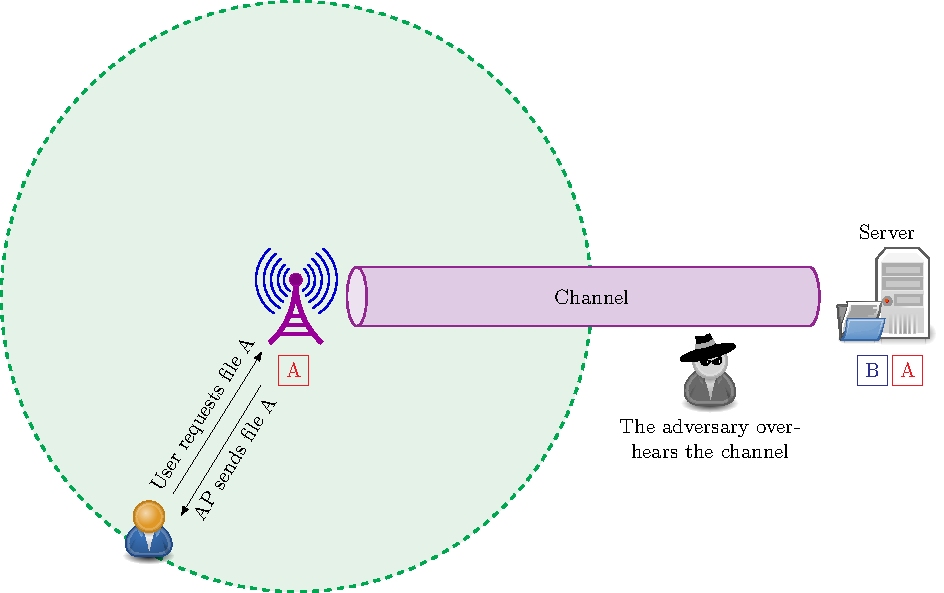
\includegraphics[width=\linewidth]{Pic/cachingSystemTotal/mainFig}
\caption{}
\label{fig:cachingSystemTotal1}
\end{subfigure}\\*[10mm]
\begin{subfigure}[b]{0.7\textwidth}\centering
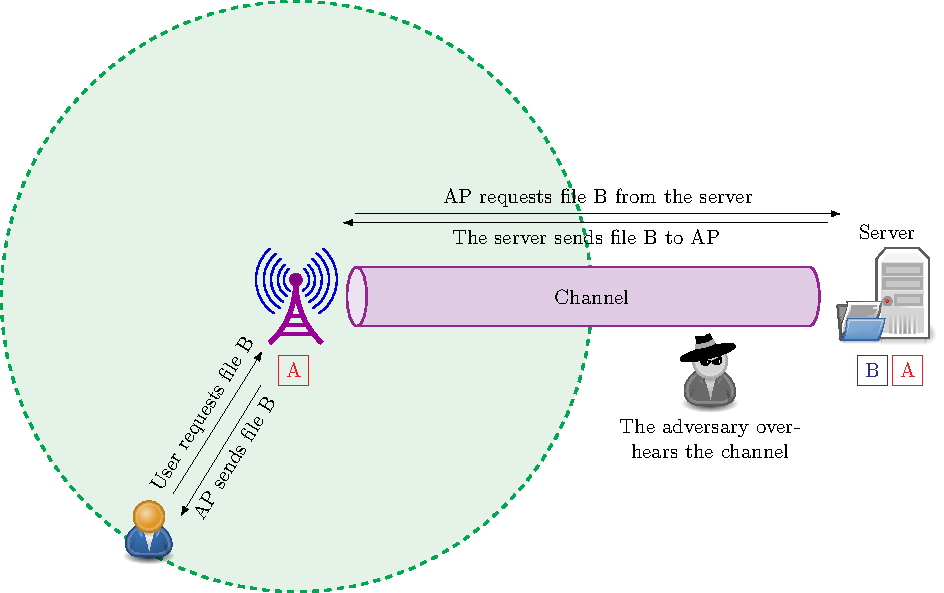
\includegraphics[width=\linewidth]{Pic/cachingSystemTotal/mainFig2}
\caption{}
\label{fig:cachingSystemTotal2}
\end{subfigure}
\caption{\lofimage{Pic/cachingSystemTotal/mainFig}
(آ)
\glsentrytext{User}
از 
\glsentryname{AP}
درخواست فایل \lr{A} را می‌کند. چون
\glsentryname{AP} در \glsentrytext{Cache}
خود این فایل را دارد، بدون درخواست از
\glsentrytext{Server}
اصلی، این فایل را به
\glsentrytext{User}
در مدت زمانی اندک ارسال می‌کند. (ب)
\glsentrytext{User}
از 
\glsentryname{AP}
درخواست فایل \lr{B} را می‌کند. چون
\glsentryname{AP} در \glsentrytext{Cache}
خود این فایل را ندارد، مجبور است  از
\glsentrytext{Server}
اصلی بخواهد که این فایل را برای او ارسال کند. با دریافت این فایل توسط 
\glsentryname{AP}
 او آن را به 
\glsentrytext{User}
می‌دهد.}
\label{fig:deliverscenarios}
\end{figure}


\end{abstract}

\section{مثال انگیزه‌بخش}
\label{sec:motivatingExample}


\section{نوآوری‌ها}
\label{sec:contributionCache}


\section{\glsentrytext{SystemModel}}
\label{sec:systemModelCaching}


\section{روش پیشنهادی}
\label{sec:proposedanaCaching}

\section{\glsentrytext{Simulation} و \glsentrytext{NumericalAnalysis}}
\label{sec:Simulation}




\chapter{\glsentrytext{Privacy}
در شبکه‌های
\glsentryname{WBSN}}
\label{chapter:WBSNPrivacy}
\begin{abstract}
امروزه شبکه‌های
\gls{WBSN}،
نقش بی‌بدیلی در
\glspl{MedicalMonitoringSystem}
ایفا می‌نماید. 
\glspl{Sensor}ی
پویش علایم حیاتی نصب شده بر بدن بیمار، موجب افزایش در کیفیت خدمات سلامت گشته است. 
\glspl{Sensor}یی نظیر \gls{EEG}, \gls{ECG}،
فشارخون، اندازه‌گیری قندخون و ....، می‌توانند در هر زمان، پارامترهای حیاتی بیماران را به صورت منظم اندازه‌گیری نمایند و آن را برای یک
\gls{SinkNode}
ارسال کنند. در این فصل خواهیم گفت که یک 
\gls{Adversary}
باهوش می‌تواند تنها با علم به نوع و زمان اندازه‌گیری هر
\gls{Sensor}
و بدون اطلاع از محتوای پیام‌های مبادله گشته، پی به اطلاعاتی در مورد بیماری فرد ببرد. 
\end{abstract}

\section{مثال انگیزش‌بخش}
\label{sec:motivatingexampleMedPrivacy}

\chapter{نتیجه‌گیری و کارهای آینده}
\label{chap:futureWork}
\begin{abstract}
در این فصل، نخست در
\autoref{sec:Conclusion}،
چکیده و نتیجه این رساله به صورت خلاصه ذکر می‌گردد. سپس در 
\autoref{sec:futureWork}،
ایده‌هایی مطرح می‌گردد که می‌تواند به عنوان ادامه پژوهش بر روی مبحث بیان شده در این رساله، در نظر گرفته شود.
\end{abstract}


\section{نتیجه‌گیری}
\label{sec:Conclusion}



\appendix
\chapter{اثبات قضایا و لم‌ها}
\section{اثبات \autoref{lemma:stabiolityproof}}
\label{sec:proofoflemmastability}
برای اثبات این لم، بدترین شرایط را در نظر گرفته و ثابت می‌کنیم که
\gls{System} 
پایداری خود را در این شرایط نیز از دست نمی دهد. پارامتر آزاد مساله 
 $\lambda_{d}^{ij}$
 است و با توجه به 
 \eqref{eq:stabilityequation}
 هر چه مقدار این پارامتر بزرگتر باشد، \gls{System} به سمت ناپایداری بیشتر سوق پیدا می‌کند. بنابراین بدترین شرایط زمانی که 
  $\lambda_{d}^{ij}$
 بیشترین مقدار خود را داشته‌باشد، و این حالت زمانی رخ می‌دهد که 
 \gls{Application} $i$ به \gls{Application} $N$ ام (\gls{Application} با بیشترین نرخ)
 نگاشته شود. به عبارت‌دیگر
$\lambda_{d}^{ij}=\lambda_{g}^{N}-\lambda_{g}^{i}$.
با قراردادن
\eqref{Eq:stabilityefffqR} در \eqref{eq:stabilityequation}
خواهیم داشت:
\begin{equation}
\frac{\lambda_{g}^{i}}{\mu_{g}^{i}} + \frac{\lambda_{d}^{ij}}{\mu_d^{ij}} =
\frac{\lambda_{g}^{i}}{\mu_{g}^{i}} +  \frac{\lambda_{d}^{ij}}{
\frac{\mu_{g}^{i}}{\mu_{g}^{i}-\lambda_{g}^{i}}\lambda_{d}^{ij}+\varepsilon} 	 \stackrel{\lambda_{d}^{ij}= \lambda_{g}^{N}-\lambda_{g}^{i}}{\Longrightarrow} 
\frac{\lambda_{g}^{i}}{\mu_{g}^{i}} +  \frac{\lambda_{g}^{N}-\lambda_{g}^{i}}{
\frac{\mu_{g}^{i}}{\mu_{g}^{i}-\lambda_{g}^{i}}(\lambda_{g}^{N}-\lambda_{g}^{i})+\varepsilon}
\label{dddsrrfgrr}
\end{equation}
بعد از مقداری ساده‌سازی 
\eqref{dddsrrfgrr}
به صورت زیر در خواهد آمد.
\begin{align}
\frac{\lambda_{g}^{i}}{\mu_{g}^{i}} +  \frac{\lambda_{g}^{N}-\lambda_{g}^{i}}{
\frac{\mu_{g}^{i}}{\mu_{g}^{i}-\lambda_{g}^{i}}(\lambda_{g}^{N}-\lambda_{g}^{i})+\varepsilon} & = 	\frac{\lambda_{g}^{i}}{\mu_{g}^{i}} + \frac{\mu_{g}^{i}-\lambda_{g}^{i}}{\mu_{g}^{i}+\varepsilon'}\nonumber\\
& < \frac{\lambda_{g}^{i}}{\mu_{g}^{i}} + 1 - \frac{\lambda_{g}^{i}}{\mu_{g}^{i}}=1.
\end{align}


\bibliography{./ETC/library}
\printglossary
\printindex

\thispagestyle{empty} %prevents tex from numbering of this page
\begin{latin} % xepersian enviorment

\centerline{\textbf{\large{Abstract}}}
\vskip 1cm
 
Recent  investigations have clarified that not only insensitive data with no encryption methods, but amazingly also encrypted sensitive data may translate into invaluable information by an intelligent adversary. In the latter case, in spite of the protection that data encryption might
provide, there are many aspects related to the creation and delivery of messages that remain
unprotected by conventional security mechanisms. Complement to the data encryption methods,
other techniques are required to protect such contextual information to preserve the privacy of the
sources and have been the focus of attention of many research studies during the past few years. The former is known as data-oriented privacy and employs encryption methods to
protect data, while the latter is known as context-oriented privacy, which focuses on preservation
of the contextual information such as the location and the time when a message is generated
i.e., location and temporal privacy, respectively. 
 Inhibiting the adversary of being able to extract information from the traffic rate of source nodes is a complicated task unless taking into consideration the \emph{flow conservation law} effect of the transmitter queue. A reliable method of preserving the privacy that copes with the \emph{flow conservation law}. Augmenting dummy packets, however, bears redundancy and hence requires extra resources in terms of bandwidth and buffer requirements and more importantly suggests higher transmitting energy consumption. Grounded on the queueing and information theories, in this paper we present an efficient method that minimally augments dummy packets to preserve the source rate privacy at a given degree while preserving the delay distribution of the original packets intact, and thus does not affect the QoS parameters of the transmitted data in terms of delay and jitter. Then we extend our proposed approach to preserve privacy of a general feature. We present an approach that mixes the features of applications in the source node such
that maximizes the ambiguity of adversary. Finally, we formulate a mathematical model for privacy preserving of a caching system and then present a method so as to cache
files in an efficient manner such that maximizes the degree of
privacy preservation while maintains the average delivery load at
a given level.

\end{latin}

%\makeatletter
%\newcommand{\englishcover}{
\clearpage \newpage
\thispagestyle{empty}

\begin{latin}
	\begin{center}
	\begin{table}
	\begin{tabular}{ccc}
	
\includegraphics[width=.25\textwidth]{Pic/logo2}&
	\begin{minipage}{0.5\linewidth}
	\begin{center}
	{\Large	\textbf{University of Tehran}}\\*[3mm]
	{\Large	\textbf{College of Engineering}}\\*[3mm]
{\Large	School of  Electrical and Computer Engineering}
	\end{center}
	\end{minipage}	&
	
\includegraphics[width=.2\textwidth]{Pic/logo} \\
& & \\
& & \\
& & \\
	\end{tabular}
	\end{table}

		\begin{center}
			\huge{Analysis of privacy preserving in the communication networks using queuing theory}
		\end{center}
		\vskip 2.1cm
		\Large{By:}         \\ [0.2cm] 
		\Large{{Abolfazl Diyanat}}
		\vskip 1.5cm
		\Large{Supervisor:} \\[0.2cm]   \Large{{Dr. Ahmad Khonsari}}
		\vskip 1.5cm
		\large{A thesis submitted to the Graduate Studies Office in partial fulfillment of the
		requirements}\\*[5pt]
		\large{ for   the degree of doctor in }\\*[5pt]
			 \large{
			 Computer Engineering - Software}
		\vskip 1.7cm
		\Large{December 2016}
\end{center}
\end{latin}
%}
%\makeatother
\end{document}
